\documentclass[preprint,5p,authoryear]{elsarticle}

\usepackage{amsmath}
\usepackage{amsfonts}
\usepackage{graphicx}
\usepackage[small]{caption}
\usepackage[subrefformat=parens]{subcaption}
\usepackage{booktabs}
\usepackage{multirow}
\usepackage{rotating}
\usepackage{url}
\usepackage[table]{xcolor}
\usepackage{hyperref}
\usepackage{dblfloatfix}

\journal{NeuroImage}

\bibliographystyle{elsarticle-harv}

\begin{document}

\begin{frontmatter}

\title{Identifying virtual-world stimulus information from fMRI data}

\author[UT]{Andrew Floren\corref{cor}}
\ead{afloren@utexas.edu}

\author[UT]{Bruce Naylor}

\author[UT]{David Ress}

\address[UT]{The University of Texas at Austin, Austin, TX 78712 USA}

\cortext[cor]{Corresponding author.}

\begin{abstract}
abstract
\end{abstract}

\begin{keyword}
keyword1 \sep keyword2
\end{keyword}

\end{frontmatter}

\section{Introduction}
Much research using functional magnetic resonance imaging (fMRI) and the blood oxygen level dependent (BOLD) signal utilize static images to analyze how the brain responds to stimuli.
Such work usually focuses on a single variable of interest, and creates stimuli that attempt to isolate that variable.
While this has proven to be a successful approach, it does not mimic the dynamically changing environment in which the primate brain has evolved.
More natural and dynamic stimuli will evoke a more complex network of brain responses.
These complex responses can make interpretation difficult, yet it is important to test whether currently accepted neural correlates of experience remain valid in more natural settings because the context in which a stimuli is presented will affect how it is processed.

Researchers have been using dynamic stimuli in the form of virtual reality (VR) environments \citep{Maguire1998,Calhoun2002,King2006,Mathiak2006,Spiers2007a,Hassabis2009} and prerecorded movies \citep{Hasson2004,Chadwick2010,Nishimoto2011} for some time.
VR stimuli have a two strong advantages over prerecorded movies: the stimulus designer has complete control over the stimuli and the subject can interact with the VR environment in real time.
Precise control of the VR environment allows for the interrogation of very subtle parameters as well as automatic coding of the scene.
Many variables of interest, such as semantic labels for visible objects are explicitly specified by the VR design, avoiding the need to manually label each frame as is usually done to analyze experiments employing movies.
Furthermore, VR permits real-time interaction that enable the examination of feedback and learning mechanisms in a realistic context.

More complex stimuli require more complex analysis methods.
In \cite{Spiers2007}, the authors review a number of experiments that use either movies or VR and discussed the wide variety of methods used to interrogate these dynamic stimuli: general linear models (GLM) including statistical parametric mapping (SPM), independent component analysis (ICA), reverse correlation, and multi-voxel pattern analysis (MVPA) being among the most popular.
These analysis methods can generally be split into stimulus-driven methods---such as SPM---which measure the statistical significance of a hypothesis, and data-driven methods---such as MVPA---which look for patterns in the fMRI signal.
Stimulus-driven analyses provide more easily interpretable results but become less and less tractable as the complexity of the stimulus increases.
Data-driven analyses, on the other hand, can cope with more complex stimuli but are more difficult to relate to brain physiology.
Data-driven analyses can be used to uncover complex patterns evoked by realistic stimuli. The observed relationships can then be used to help formulate hypotheses and design stimuli to be tested by stimulus-driven analyses. However, it may also be possible to utilize the use these realistic stimulus-response relationships to better understand subject training and pathophysiology.

Although many dynamic stimuli experiments employ GLM methods \citep{Maguire1998,Calhoun2002,King2006,Mathiak2006,Spiers2007a}, there is a general trend in newer experiments to use MVPA \citep{Hassabis2009,Chadwick2010,Haxby2001,Mitchell2003,Haynes2006}. The application of MVPA analysis to VR stimuli can open up an exciting range of experiments to examine complex brain responses in more realistic stimulus scenarios.
MVPA has been used as a blanket term for the application of any classification algorithm to fMRI data, although the support vector machine (SVM) is by far the most popular choice.
When applying MVPA, the stimulus is typically organized into multiple categories or classifications such as the presentation of houses or faces.
The algorithm is then trained to classify the pattern of BOLD activation into these categories at a particular time-point using labeled examples.
The performance of the classifier is defined to be the probability that it will successfully classify a previously unseen example;
this measure of performance must be estimated using statistical methods.
MVPA can be applied to the whole brain as well as to small localized regions such as in the ``searchlight'' technique \citep{Kriegeskorte2006} which can be used to localize functional processing.
MVPA methods consider the pattern of activation of many voxels at a particular interval in time, in contrast to GLM, which treats each voxel independently as a time-series of responses over an extended period of time.
By considering multiple voxels simultaneously, MVPA has been used to identify effects that had previously seemed too fine scale to resolve with fMRI \citep{Kamitani2005,Hassabis2009}.

Here, we test the feasibility of extracting complex information from fMRI data while subjects view natural and dynamic stimuli.
Our experiment was structured to identify those parts of the brain that are related to the perception and apparent number of human characters in a scene.
Unlike previous experiments that examined the neural correlates of object counting or number evaluation \citep{Dehaene1999,Rickard2000,Barth2006}, we used a passive-viewing VR stimulus paradigm.
To analyze the fMRI data from our more complex stimuli, we employed MVPA.
More specifically, we tested two different machine learning algorithms: the support vector machine (SVM) and feedforward neural network (NN).
These classifiers were trained using a spatially distributed subset of stimulus-responsive voxels at each time point and their performance was estimated using cross-fold validation. We carefully examined a variety of temporal splitting schemes to assess their effect on classifier performance.
Our classification accuracy was 3--4 times better than chance for all subjects and both machine-learning techniques tested.
We then utilized a novel sensitivity mapping technique to identify voxels that are important for classification and are thus likely involved in processing the information that the classifiers were trained to identify.
Results indicate that information regarding  the number of visible characters in a complex stimulus is largely encoded fairly early in visual processing, utilizing both ventral and dorsal visual streams.
The results demonstrate that complex information can effectively be extracted from a realistic VR stimulus paradigm, opening up new prospects for the use of VR with MVPA in neuroscience.


\section{Methods}

\subsection{Subjects}
Five adult males, with normal or corrected-to-normal vision, participated in the experiments. 
All subjects participated in two MRI sessions with 36 minutes of fMRI acquisition. 
An additional session was performed to acquire a high-resolution structural anatomy for each subject. 
Informed consent was obtained from all subjects.

\subsection{Stimulus}
To facilitate designing our VR stimulus, we used the Unreal Developer's Kit developed by the company Epic Games (available at \url{http://www.unrealengine.com/udk}).
This development kit is available free of charge for non-commercial applications and uses the same rendering and game engine found in many current and popular video games.

\begin{figure*}
\centering
\begin{subfigure}{0.3\textwidth}
\centering
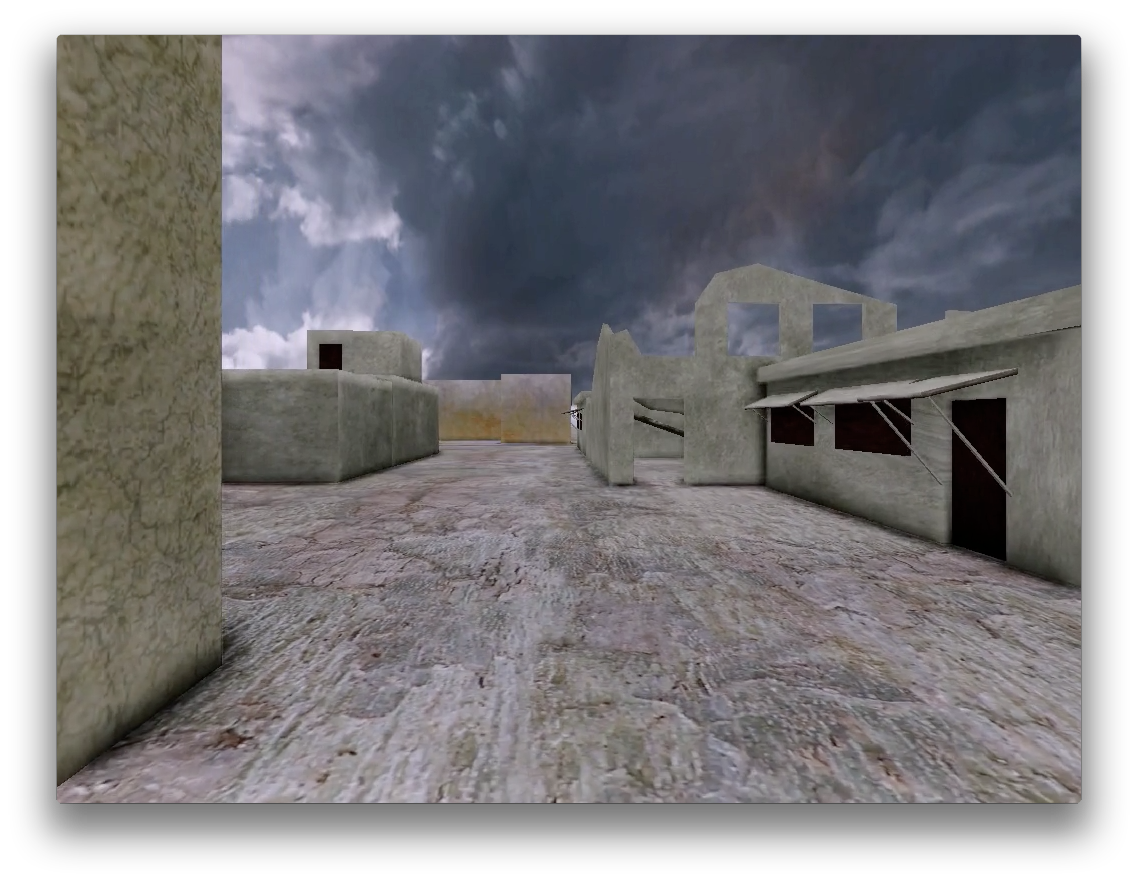
\includegraphics[width=\textwidth]{figures/stimulus-town}
\caption{}
\label{fig:stimulus-town}
\end{subfigure}
\begin{subfigure}{0.3\textwidth}
\centering
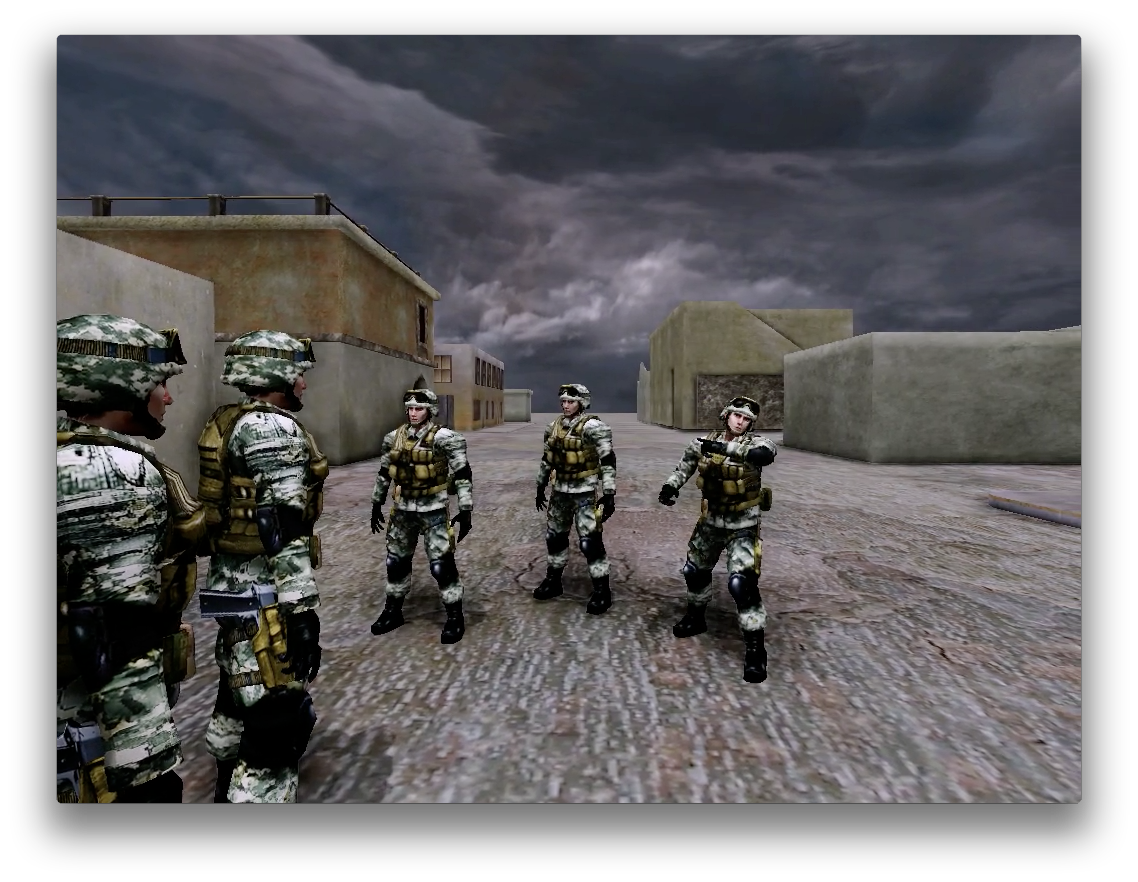
\includegraphics[width=\textwidth]{figures/stimulus-five-soldiers}
\caption{}
\label{fig:stimulus-five-soldiers}
\end{subfigure}
\begin{subfigure}{0.3\textwidth}
\centering
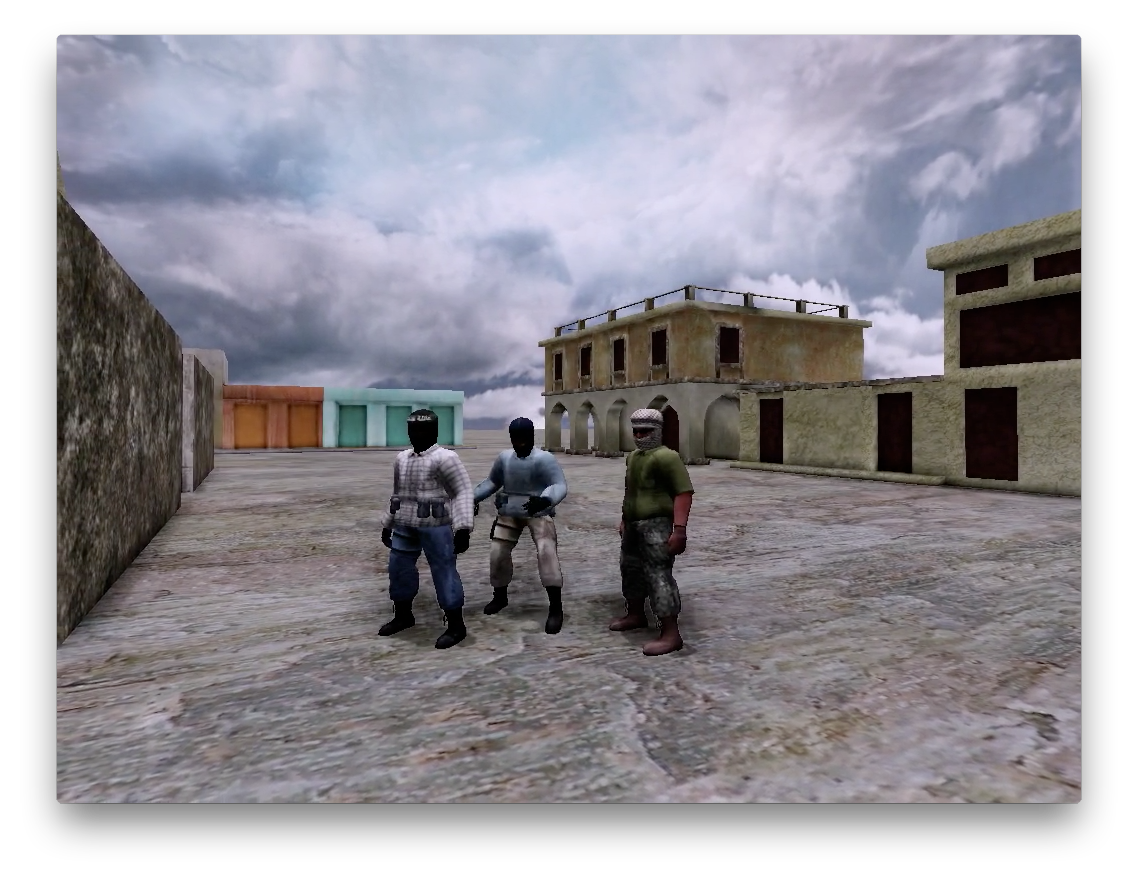
\includegraphics[width=\textwidth]{figures/stimulus-three-insurgents}
\caption{}
\label{fig:stimulus-three-insurgents}
\end{subfigure}
\caption{
\subref{fig:stimulus-town} An example frame from the stimulus where the camera is travel through the virtual environment with no characters presented.
\subref{fig:stimulus-five-soldiers} An example frame from the stimulus while characters are being presented.
\subref{fig:stimulus-three-insurgents} Another example frame from the stimulus while characters are being presented.
Note how the locations of the characters varies considerably between these two frames.}
\label{fig:stimulus}
\end{figure*}

Given our long-term interest in PTSD, we created a virtual town intended to mirror the kinds of real-world settings encountered by our military forces (see figure \ref{fig:stimulus}).
Virtual characters representing friendly forces and hostile combatants were situated at a variety of locations throughout the virtual town.
The stimulus was rendered in real-time from the point of view of a camera moving at eye level through the town. 

During the stimulus presentation, the camera followed a preset path through the town.
The stimulus employed a blocked approach. The camera would be steadily moving for 15 seconds, followed by 15 seconds in which it stopped to view virtual characters at predefined locations.
There were 4 different predefined character-viewing locations, and the number of characters present at each of these locations varied from 1 to 6 (Figs. \ref{fig:stimulus-five-soldiers} and \ref{fig:stimulus-three-insurgents}).
While the camera was stopped to view the characters, the view slowly panned and rotated and the characters engaged in animated movement sequences, so that the scene was never static.
We employed a passive viewing paradigm for this stimulus: there was no fixation dot and no instructions were given as to what to pay attention to during the presentation.

Scanning sessions included 5--6 runs that were 6 minute in duration.
Each run contained 12 alternations between moving through the virtual environment and character presentations. 
Since there were 4 predefined character viewing locations, the camera made 3 laps around the town during a single run.
While the number of characters presented in each block varied from 1 to 6, the stimulus was controlled such that a presentation with a particular number of characters appeared twice in each run.
The ordering of the presentations was also controlled such that presentations with the same number of characters were located at different viewing points.
The order of the presentations was generated randomly given the previous constraints, but the same ordering was used for each subject.
A single type of character (friends or foes) was presented in each run. 
The character type presented was alternated for each run.

\subsection{MRI protocols}
Imaging was performed on a GE Signa Excite HD scanner using the product 8-channel head coil.
We collected whole-brain image volumes using a custom GRAPPA-accelerated EPI sequence \citep{Griswold2002}. 
Sequence parameters were g-factor = 2,  TE = 25 ms, TR = 2.5 s, and  2.5-mm cubic voxels across a 200 mm field-of-view. 
The slice prescription included 40 slices oriented along the AC-PC axis. 
A high-order shim was  performed to improve field homogeneity.

A set of T1-weighted structural images was obtained on the same prescription at the end of functional acquisition session using a three-dimensional (3D) fast RF-spoiled GRASS (fSPGR) sequence. 
These anatomical images were then used to align the functional data to a structural 3D reference volume, which was acquired for each subject in a separate session. 
The structural reference volume was T1-weighted with good gray-white contrast and was acquired using a 3D, inversion-prepared, fSPGR sequence (minimum TE and TR, TI = 450 ms, 15$^\circ$ flip angle, isometric voxel size of 0.7 mm, 2 excitations, $\sim$28-minute duration).

\subsection{Preprocessing}
Preprocessing of the fMRI data was performed using the mrVista software package (available for download at \url{http://vistalab.stanford.edu/}) as well as additional tools developed on the mrVista framework in our lab. 
The first 15 seconds of data  were discarded to reduce transient effects.
We then estimated in-scan motion using a robust intensity-based scheme \citep{Nestares2000}. 
Between-run motion was corrected using the same scheme, this time applied to the temporal average intensity of the entire scan. 
The first run of the session was used as the reference. 
Additionally, we applied a Wiener filter deconvolution \citep{Poor1980} using a generic difference-of-gamma HRF \citep{Glover1999} as the kernel to shift the peak response in time so that it is aligned with its associated stimulus.
We are interested in learning associations between patterns of activation in the brain and stimulus presentation so it is important that the activation is properly aligned temporally with the stimulus.

Wiener filter deconvolution can be summarized as follows:
Given a system
\begin{equation}
y(t) = h(t) \ast x(t) + n(t)
\end{equation}
where $x(t)$ is the signal of interest, $h(t)$ is some blurring kernel, $n(t)$ is independent additive noise, and $y(t)$ is the recorded signal.
We want to find the deconvolution kernel $g(t)$ such that 
\begin{equation}
\hat{x}(t) = g(t) \ast y(t)
\end{equation}
minimizes the mean squared error between $x(t)$ and $\hat{x}(t)$, or
\begin{equation}
\sum_{t}{\left( \hat{x}(t) - x(t) \right)^{2}}
\end{equation}
The solution for the optimal $g(t)$ is most easily expressed in the Fourier domain.
\begin{equation}
g(t) \xrightarrow{\mathcal{F}} \frac{H^{*}(f)}{\left|H(f)^{2}\right| + \mbox{SNR}^{-1}(f)}
\end{equation}
Where $\mbox{SNR}(f)$ is the signal to noise ratio $\frac{\left| X(f) \right|}{\left| N(f) \right|}$.

\begin{figure*}
\centering
\begin{subfigure}{0.3\textwidth}
\centering
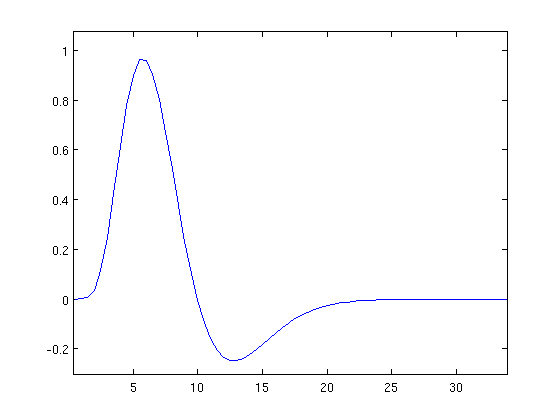
\includegraphics[width=\textwidth]{figures/hrf}
\caption{}
\label{fig:wiener-hrf}
\end{subfigure}
\begin{subfigure}{0.3\textwidth}
\centering
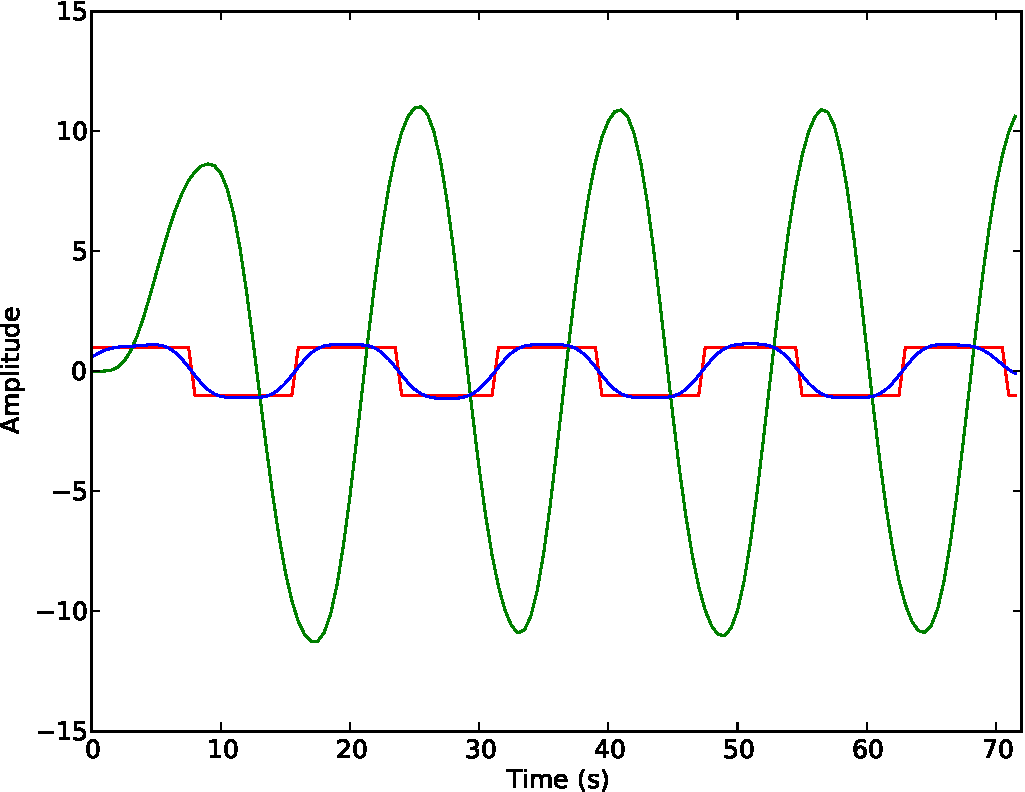
\includegraphics[width=\textwidth]{figures/square-wiener-deconvolution}
\caption{}
\label{fig:wiener-square}
\end{subfigure}
\begin{subfigure}{0.3\textwidth}
\centering
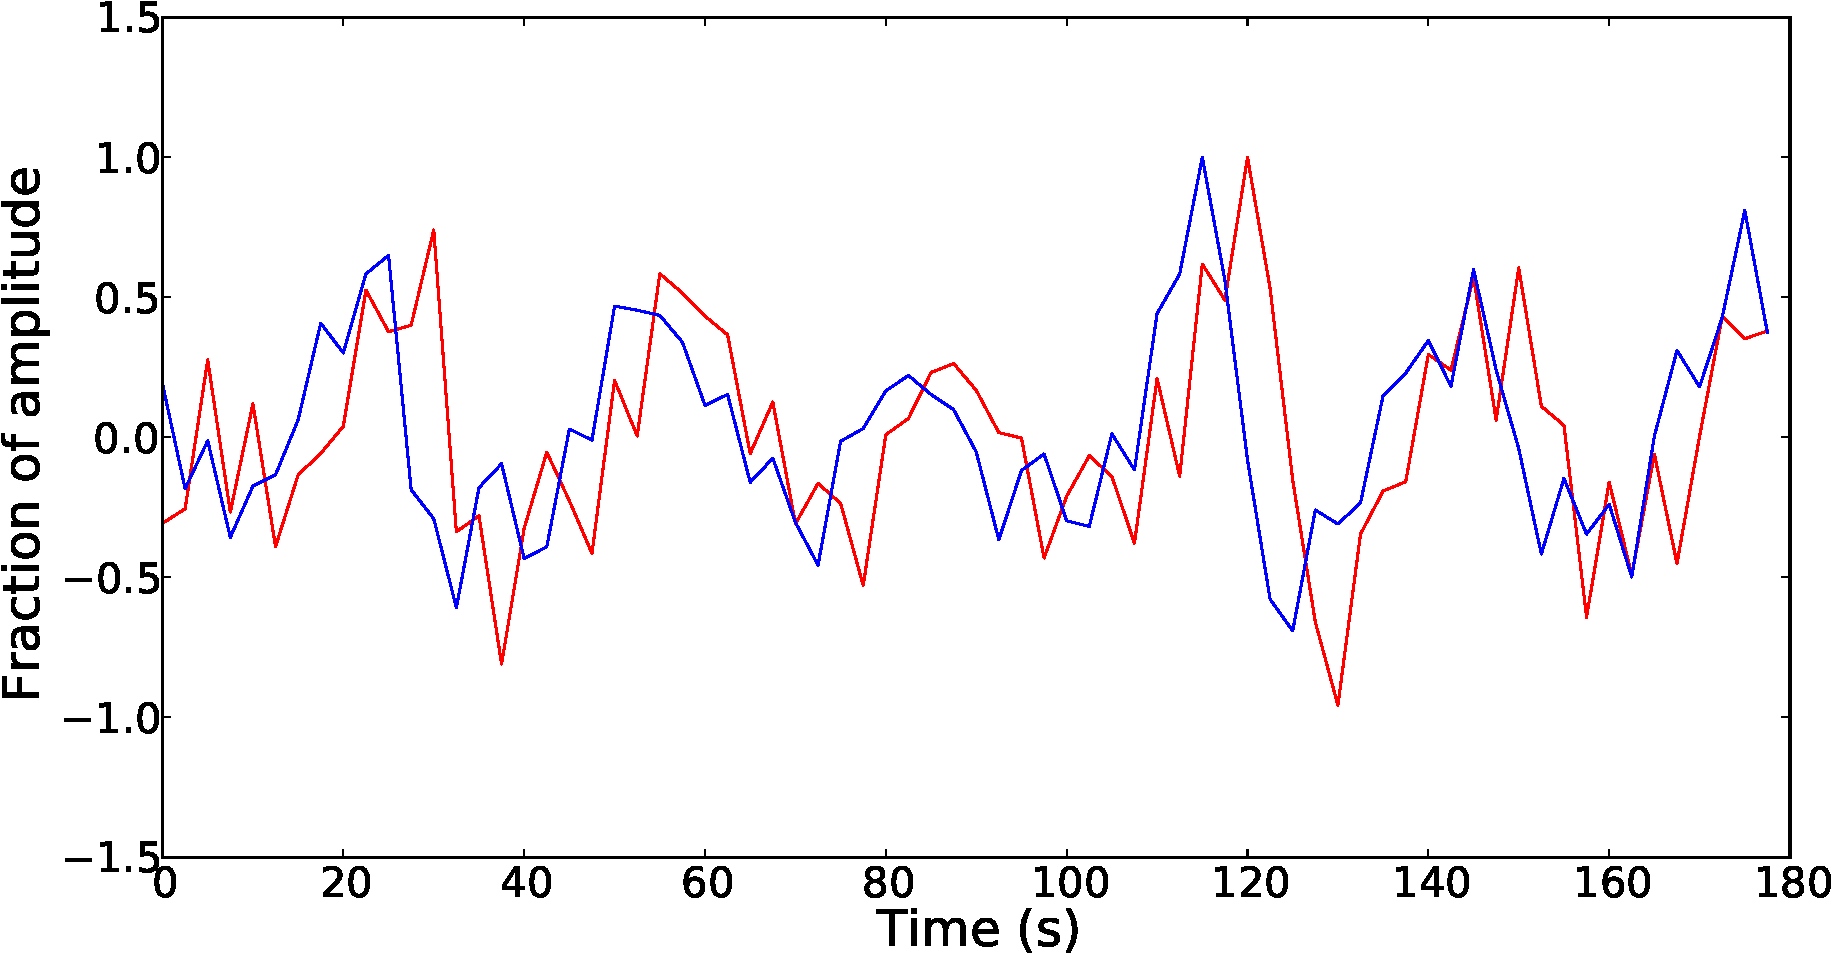
\includegraphics[width=\textwidth]{figures/voxel-wiener-deconvolution}
\caption{}
\label{fig:wiener-voxel}
\end{subfigure}
\caption{
\subref{fig:wiener-hrf} The difference-of-gamma HRF employed as $h(t)$. 
\subref{fig:wiener-square} A simple square wave in red. 
The same square wave after convolution with $h(t)$ in green, then after Wiener-filter deconvolution in blue. 
\subref{fig:wiener-voxel} An example voxel time series in red. 
The same time series after Wiener-filter deconvolution in blue.}
\label{fig:wiener-deconvolution}
\end{figure*}

In fMRI, $y(t)$ is the recorded BOLD signal, $h(t)$ is the hemodynamic response function, and $x(t)$ is the neural response.
Calculating $g(t)$ requires estimates of the power spectral density of the signal of interest as well as the noise.
However, the noise $n(t)$ corresponds not only to scanner noise but other nuisance factors such as pulse and respiration.
This makes modeling the noise, and its power spectral density, very difficult.
Therefore, we set $\mbox{SNR}(f) = 1$% for all frequencies $f$. This has the effect of largely removing the hemodynamic delay without much noise increase (Fig. \ref{fig:wiener-deconvolution}.

The high-resolution reference anatomies were segmented using the Freesurfer image analysis suite to create approximate parcellations of the gray matter in each subject, as well as a surface model useful for visualization of the results.
Freesurfer is documented and freely available for download online (\url{http://surfer.nmr.mgh.harvard.edu/}).

\subsection{Dimensionality reduction}
When performing MVPA, each voxel can be thought of as corresponding to a separate dimension of a very high-dimensional space.
In our case, the number of voxels/dimensions was typically $80 \times 80 \times 40 = 256,000$.
Unfortunately, the number of examples necessary to train a classifier increases exponentially with the number of dimensions.
Therefore, as a preprocessing step before applying our machine learning algorithms we needed to reduce this dimensionality.
This not only speeded up both training and classification but could also improve the performance of the resulting classifiers.

Principal component analysis (PCA) is a very common tool for dimensionality reduction \citep{Hotelling1933}.
However, PCA only selects the orthogonal dimensions with the highest variance which is very likely to be noise and is therefore not well suited for fMRI analysis.
A univariate statistic, as typically used in  fMRI analysis,can also be a good candidate for selecting voxels \citep{Norman2006,Pereira2009}.
While effective, these methods were not designed for feature selection and many of them make a number of assumptions about the data such as Gaussian statistical distribution.
We have developed a method of dimensionality reduction, which we call harmonic analysis, that selects voxels that are driven most strongly by the 30-second duty cycle of our block design.
This method is similar to other univariate statistics but the only assumption it makes is that the BOLD response is linear with respect to the stimulus.
The primary advantage  of harmonic analysis over other univariate statistics is that it can detect voxels that covary with the stimulus regardless of their detailed temporal relationship. Thus, it includes voxels that respond positively to either the character-presentation or motional phases of the stimulus alternation, or to more complex patterns such as a brief strong response to both phases. All repetitive responses that follow the period of the stimulus alternation are included by this method, minimizing any bias in the dimension reduction.
Harmonic analysis take advantage of the fact that the response of any linear system to a blocked alternation at frequency $f$ will contain power only at $f$ and its harmonics. 
Under a linear response assumption, we can therefore form an unbiased estimate of the response power by summing the power at these frequencies. 
Let $y(t)$ be the recorded discrete time series at some voxel.
Then let $Y(f)$ be the discrete Fourier transform of $y(t)$.
The fractional harmonic power of that time series is defined as:
\begin{equation}
P_h = \frac{\sum_{i = 1}^{M}{\left|Y(i \cdot N)\right|^{2}}}{\sum_{f}{\left|Y(f)\right|^{2}}}
\end{equation}
Where $P_h$ is the fractional harmonic power, $M$ is the number of harmonics, and $N$ is the frequency of interest, in our case the period of the block alternations. 
Because the BOLD response has a predominantly low-pass temporal frequency response, we can accept $M = 4$. 
Using $P_h$, we then selected a particular number $N$ (typically 2000) voxels with the greatest power. 

This harmonic-power selection was based on the alternation between characters present and characters absent, without regard to the number of characters presented. 
Therefore, we will only be presenting classifier accuracy estimates for character count, and not for the presence or absence of characters to avoid cross-contamination between dimension-reduction and  classification criteria that would result in inflated classifier performance estimates \citep{Pereira2009}.
However, as a check we built classifiers to distinguish between time points with and without characters, and their performance was consistently above 95\%, confirming the proper operation of our machine-learning algorithms.

\subsection{Classification}
Using the time series from the voxels selected by the harmonic analysis, we trained a linear SVM \citep{Cortes1995} and a feedforward neural network \citep{Hornik1989,Hagan1994}.
To maximize our temporal resolution, each 2.5-second frame (time point) was treated as a separate example, rather than aggregating across the 15-second blocks.

To measure the significance of the results and to compare the SVM and NN we must have a measure of their performance.
The performance of machine learning algorithms is generally defined to be the expected accuracy of the classifier on a previously unseen example \citep{Bishop2006}.
In practice, this measure of performance can only be estimated.
This is commonly achieved by first splitting the available examples into a training and test sets.
Then, the performance is estimated as the average accuracy of the classifier on the test set after having been trained on the training set.
In practice, the process of splitting all of the available examples into training and test sets is performed multiple times to reduce the variance of the performance estimate.
This procedure is known as cross-fold validation \citep{Kohavi1995} where each split of the data into training and test sets is called a ``fold''.

The SVM finds the hyperplane in the high-dimensional input space that separates examples from different classes with the greatest margin \citep{Cortes1995}.
A simple SVM can only discriminate between two classes.
However, it is possible to combine multiple SVMs to discriminate between more than two classes.
The two most common approaches to building a multi-class SVM are one-versus-all and one-versus-one \citep{Weston1999}.
In one-versus-all, SVMs are trained to distinguish between a particular class and all examples not from that class.
In one-versus-one, SVMs are trained to distinguish between every possible combination of classes.
For $N$ classes, one-versus-all classifiers require training $(N-1)$ SVMs while one-versus-one classifiers require training $(N-1)(N-2)$ SVMs.
Although the performance of these two approaches is generally similar, we have used the one-versus-one approach because we found its performance to be superior for our application.

Feedforward neural networks trained via back propagation learn to approximate functions using compressive non-linearities \citep{Hagan1994}.
Any function (including non-linear and discontinuous functions) can be approximated to an arbitrary degree given a sufficient number of hidden units \citep{Hornik1989}.
Precisely because of this flexibility, feedforward neural networks are prone to overfitting.
That is, the network perfectly encodes the training examples at the expense of poor performance on the test examples.
For this reason, the feedforward neural network further subdivides the training examples into training and validation sets.
The validation set is used to determine when the network has begun overfitting the training examples and ceases iteration.

Previous studies have discussed issues with optimistically biased performance estimates due to temporal correlations violating independence assumptions between training and test set samples \citep{Pereira2009}. The slow speed of the fMRI hemodynamic response clearly introduces temporal correlations on time scales less than 15 seconds.
For our data, artificial correlations occurred when the random sampling that divides the data into the different sets yields training and test samples from the same (15 sec) block.

This raises a more general question: what is the relationship between performance estimates and temporal correlation?
To explore this, we estimated classifier performance using 5 different methods for splitting the training and test examples in order to vary the average temporal distance between frames in the two sets. 
The first four methods deal only with frames from a particular session.
In the first method, which we will refer to as  ``frame split", frames were independently drawn into the training and test sets. 
Although the draws were independent, there is no restriction to prevent adjacent frames being split between the training and test sets.We expect this method to exhibit artificially high performance because of the aforementioned temporal correlation of the slow fMRI data.
In the second method, which we will refer to as ``block split", sets of frames corresponding to the 15 sec. blocks were independently drawn into the training and test sets.
In our third method, we exploit the fact that each 6 min run cycles through all combinations twice, but in a different order the second time.
Accordingly, sets of frames were independently drawn from these half-runs, referred to as ``half-run split". 
In our fourth method, termed ``run split", entire 6-min runs of frames were independently drawn. 
Table \ref{tab:training-split} summarizes these training and test set split methods and the temporal separations between the training and test data for single runs. Because the randomization extends across the entire the entire run, the mean temporal separations do not vary much between the various splits. The differences in the temporal distributions are therefore characterized by the mean (across folds) of their median values, which vary from ?? s (frame split) to ??? s (run split)and the mean of their minimum delay, which varies from $\sim$3 s (frame split) to 130 s (run split).
And finally, we tested a fifth method, termed ``session split", where we used one entire session for training and a second session for test.
This method is similar to measures of between-session classifier accuracy used in \citep{Haynes2005}.

%\begin{figure*}
%\centering
%\begin{subfigure}{0.3\textwidth}
%\centering
%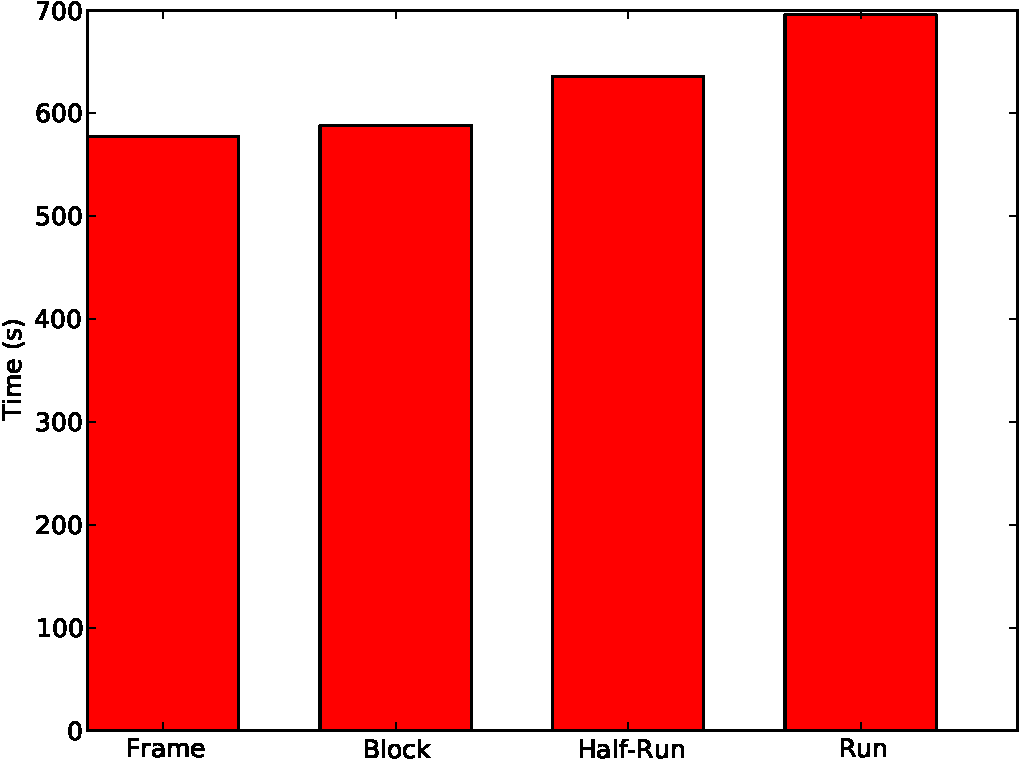
\includegraphics[width=\textwidth]{figures/mean-delay-graph}
%\caption{}
%\label{fig:mean-delay-graph}
%\end{subfigure}
%\begin{subfigure}{0.3\textwidth}
%\centering
%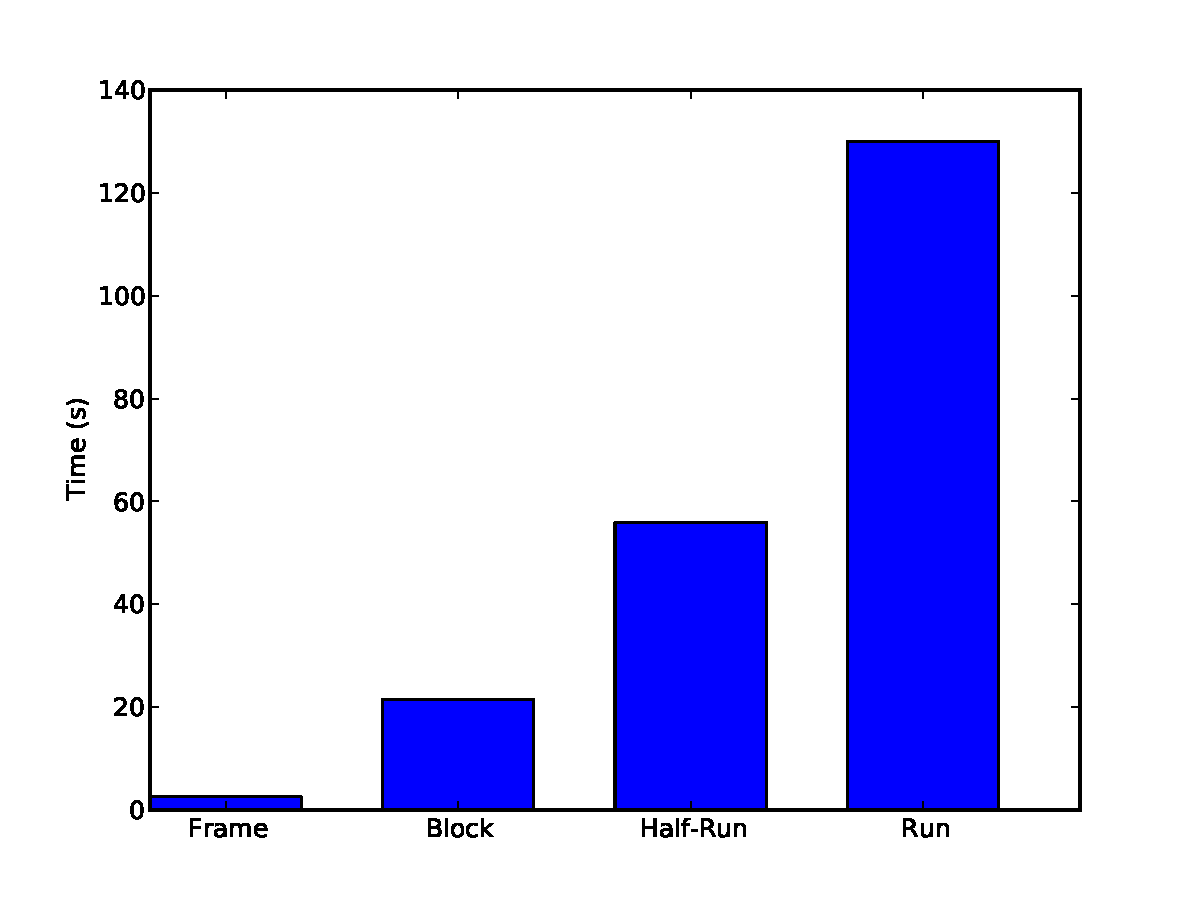
\includegraphics[width=\textwidth]{figures/min-delay-graph}
%\caption{}
%\label{fig:min-delay-graph}
%\end{subfigure}
%\caption{The \subref{fig:mean-delay-graph} mean delay and \subref{fig:min-delay-graph} minimum mean delay between examples in the train and test set for four of the split methods. 
%The session split method is excluded because both the mean and minimum delay are much larger than the other splits and the delays vary significantly between subjects.}
%\end{figure*}

\begin{table}
\centering

\begin{tabular}{l*{2}{c}}
\toprule
Split & Mean Delay & Mean Minimum Delay \\
\midrule
Frame & 5776 & 26 \\
Block & 5883 & 215 \\
Half-Run & 6360 & 559 \\
Run & 6960 & 1300 \\
Session & 0 & 0 \\
\bottomrule 
\end{tabular}

\caption{Summary of training and test set split methods and the mean temporal delay between the training and test data.}
\label{tab:training-split}
\end{table}

For the frame and block splits, the classifier performances were estimated using 10-fold cross-validation.
That is, the dataset was randomly split into the training and test sets 10 times and a classifier is trained on each split.
The classifier's performance is then estimated as the average of its performance across all 10 splits.
For the half-run, run, and session splits, only 8, 4, and 2 unique splits are possible, respectively, due to the much smaller number of runs and sessions per subject. 
Therefore, only 8-fold, 4-fold, and 2-fold cross-validation were employed for estimating classifier performance on these splits.

We define the classifier's overall performance or accuracy to be the probability that it will correctly classify a previously unseen time-slice.
As such, this measure of performance can only be estimated by dividing the number of correctly classified examples in the test set by the total number of examples in the test set.
We can also discuss classifier performance with respect to a single class.
Single class performance is traditionally measured along two axes: \emph{precision} and \emph{recall}.
\emph{Precision} with respect to class $c$ is the probability that a previously unseen data point was classified correctly given that it was classified as $c$.
\emph{Recall} with respect to class $c$ is the probability that a previously unseen data point was classified correctly given that it is actually a member of $c$.
Again, these measures can only be estimated from the test set.
$\mbox{\emph{precision}} = tp / (tp + fp)$, where $tp$ is the number of true positives and $fp$ is the number of false positives.
$\mbox{\emph{recall}} = tp / (tp + fn)$, where $fn$ is the number of false negatives.

Another tool for examining classifier performance is the confusion matrix.
If $\mathbf{C}$ is a confusion matrix, then the value of $C_{ij}$ is equal to the number examples of class $i$ that were classified as class $j$.
Therefore, values along the diagonal of a confusion matrix correspond to correct classifications while other values correspond to incorrect classifications.
The confusion matrix also simplifies estimating precision and recall for each class.
The value of $C_{ii}$ divided by the sum of all values along row $i$ is the estimate for the recall of the $i^{th}$ class.
Similarly, the value of $C_{jj}$ divided by the sum of all values along column $j$ is the estimate for the precision of the $j^{th}$ class.
Finally, overall classifier performance can be estimated by dividing the sum along the diagonal, or the trace, by the sum of the entire matrix.

\subsection{Sensitivity Analysis}
MVPA can tell us whether the time-series data from a subset of human brain voxels is discriminative with respect to the stimulus being classified. 
However, these results do not show which voxels in the large group were actually important for that discrimination.
This information is important for localizing functions in the brain.
One existing technique is to train machine learning classifiers on small localized areas in the brain and use their performance as a measure of the strength of the function in question in that area.
This is known as the ``searchlight'' technique \citep{Kriegeskorte2006}.
While this technique is effective for simple highly localized functions, the results are less clear when the function is sparsely distributed over the brain.
No one region may contain enough information for accurate predictions.

To overcome this limitation, we have trained our classifiers on all stimulus-responsive regions of the brain and used a neural-network sensitivity analysis to display the spatially distributed set of voxels that are the most important for identifying the classes.
Specifically, we calculate the sensitivity, or magnitude of change, of the output of the classifier with respect to a change in each voxel
 \citep{Zurada1994}.
Let $\mathbf{o}$ be the vector of outputs and $\mathbf{x}$ be the vector of inputs.
Then the sensitivity of output $k$ to input $i$ is defined by:
\begin{equation}
S_{ki} = \frac{\delta o_{k}}{\delta x_{i}}
\end{equation}
which is simply the partial derivative of the output with respect to the input.
If we let $\mathbf{w}$ be the weight matrix from the hidden layer to the output layer and $\mathbf{v}$ be the weight matrix from the input layer to the hidden layer then the partial derivative can be expressed as follows:
\begin{equation}
\frac{\delta o_{k}}{\delta x_{i}} = o'_{k} \sum^{J}_{j=1}{w_{kj}y'_{j}v_{ji}}
\end{equation}
Where $J$ is the total number of hidden units in that layer of the neural network,  $o'_{k}$ is the value of the derivative of the activation function at output $k$, and $y'_{j}$ is the value of the derivative of the activation function at hidden neuron $j$.
Finally, the entire sensitivity matrix can be expressed in matrix notation as:
\begin{equation}
\mathbf{S} = \mathbf{O}' \times \mathbf{W} \times \mathbf{Y}' \times \mathbf{V}
\end{equation}
Where
\begin{equation}
\mathbf{O}' = diag(o'_{1},~o'_{2},~\cdots,~o'_{K})
\end{equation}
\begin{equation}
\mathbf{Y}' = diag(y'_{1},~y'_{2},~\cdots,~y'_{K})
\end{equation}
However, because the transfer functions are non-linear they can only be evaluated for specific input values.
Therefore, we calculate the average sensitivity matrix across all input vectors.
\begin{equation}
\mathbf{S}_{avg} = \sqrt{ \frac{ \sum_{n = 1}^{N}{ \left( \mathbf{S}_{n}\right)^{2} } }{N} }
\label{eqn:sensitivity}
\end{equation}
Where $N$ is the number of input vectors.
The magnitude is squared so that the effects of both positive and negative sensitivities are included in the average.
(The average of the absolute value of sensitivities could also have been employed.)
Eq. \ref{eqn:sensitivity} gives a sensitivity value for each voxel with respect to every output, whereas it is useful to have a measure of the sensitivity of a voxel with respect to any output.
We define this metric by taking the maximum sensitivity of each voxel across all outputs.
\begin{equation}
\Phi_{i} = \max_{k=1 \dots K}{S_{ki,~avg}}
\end{equation}
This sensitivity can now be projected back into the volume anatomy space to create a  map that reflects the relative incremental importance of each voxel's response to the classification decision.

To  explore the relationship between sensitivity and classifier performance we plotted the performance of the classifier when trained on only a subset of the input voxels as determined by a minimum sensitivity cut off.
This threshold was determined by iteratively retraining the neural network with successively higher thresholds.
Figure \ref{fig:sensitivity-cutoff} shows this plot together with histogram of sensitivity values for subject d.
Interestingly, the performance of the classifier was not significantly affected until a majority of the voxels have been removed.

\begin{figure}
\centering
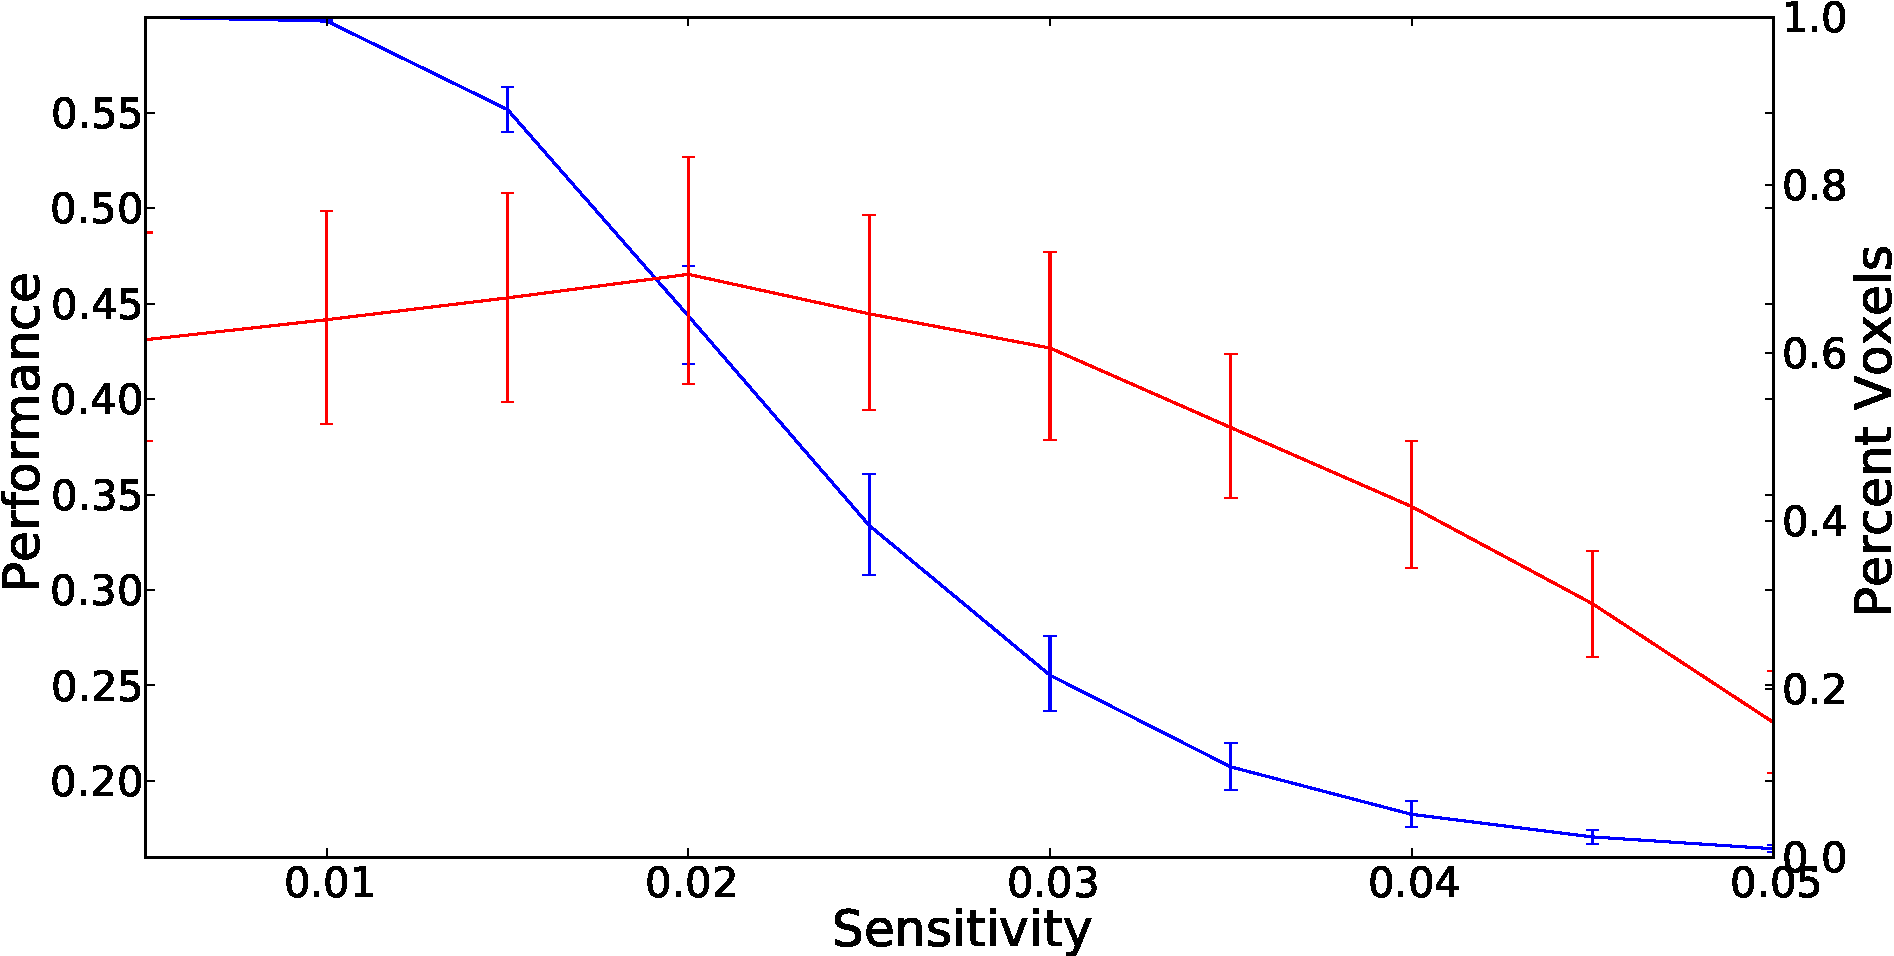
\includegraphics[width=0.3\textwidth]{figures/performance-verse-sensitivity-cutoff}
\caption{A histogram of the sensitivity analysis values and a plot of the feed forward neural network $F_1$ score when the inputs are pruned at a particular sensitivity value. }
\label{fig:sensitivity-cutoff}
\end{figure}

We employed Freesurfer image analysis suite to construct cortical surfaces for each of our subjects using high-resolution anatomy volumes.
Then, we constructed 10 anatomical labels on each surface based on FreeSurfer's automatically generated labels.
These labels are presented in figure \ref{fig:labels}.
The labels we used largely overlap with FreeSurfer's labels.
However, the label for the banks of the superior temporal sulcus was subdivided and incorporated back in to the superior and middle temporal labels.
Additionally, the supramarginal label was merged with the inferior parietal label.
For most subjects, several of the automatic labels were also edited by hand to better conform with the sulcal boundaries of the subject.
We then projected each subject's volume sensitivity map onto their cortical surface and blurred along the surface using a 5 mm full-width half-maximum (FWHM) Gaussian kernel.

\begin{figure*}
\centering
\begin{subfigure}{0.3\textwidth}
\centering
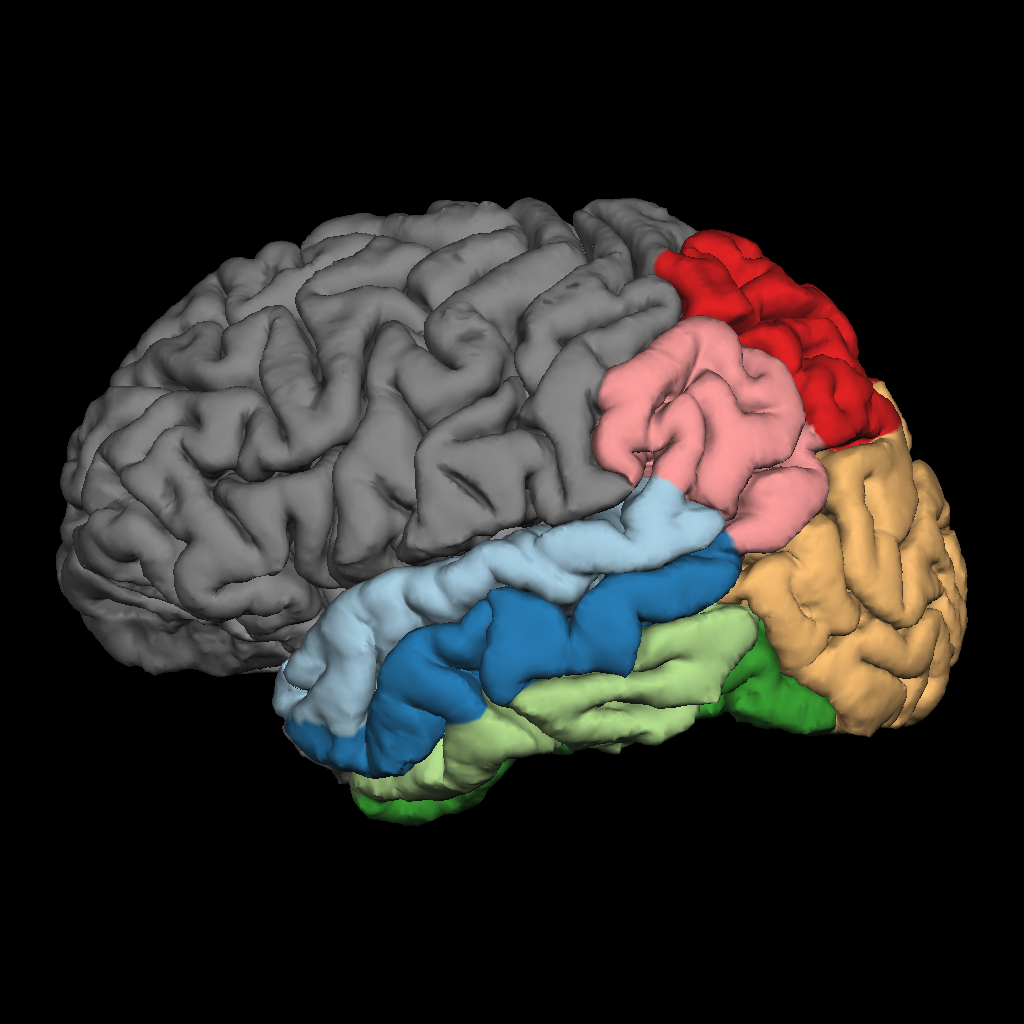
\includegraphics[width=\textwidth]{figures/lh-lateral-labels}
\caption{lateral labels}
\label{fig:leteral-labels}
\end{subfigure}
\begin{subfigure}{0.3\textwidth}
\centering
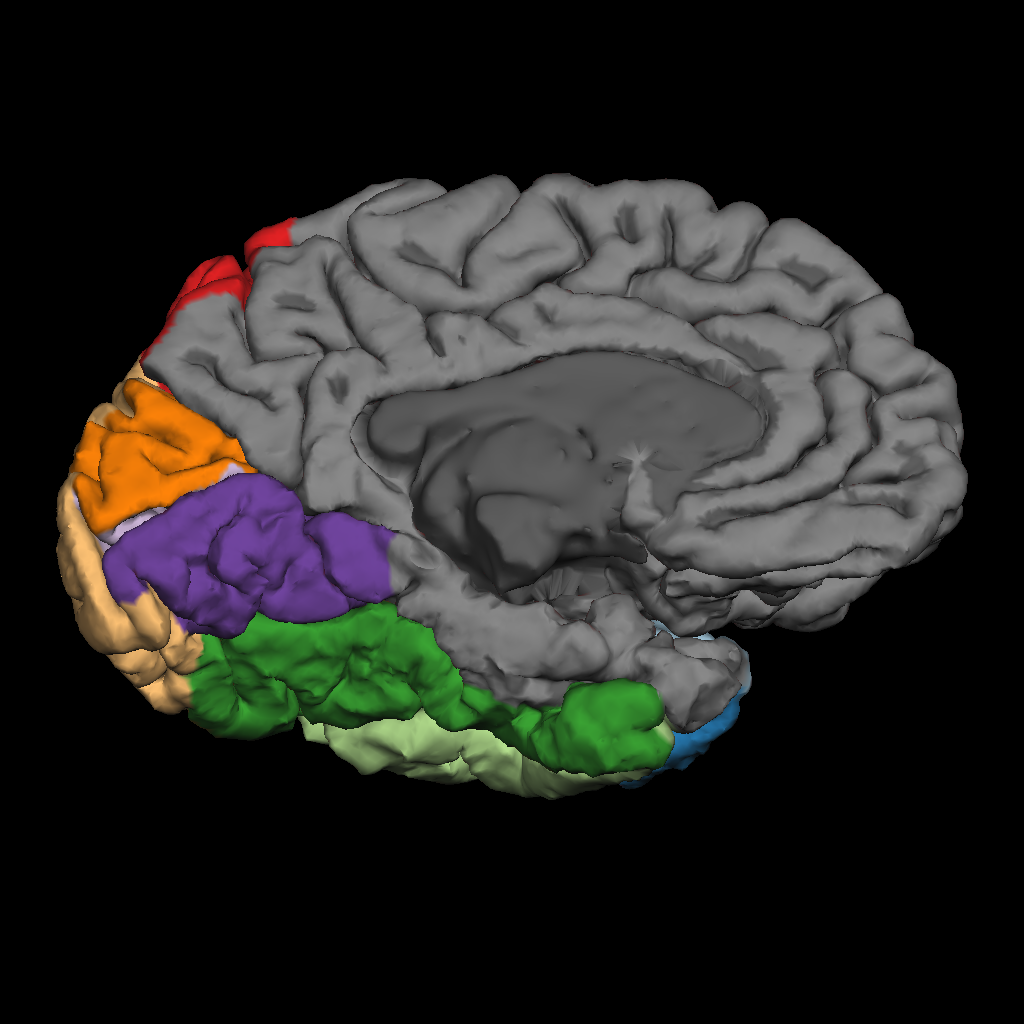
\includegraphics[width=\textwidth]{figures/lh-medial-labels}
\caption{medial labels}
\label{fig:medial-labels}
\end{subfigure}
\caption{Color coded region labels used for aggregating sensitivity results: light blue -- superior temporal, dark blue -- middle temporal, light green -- inferior temporal, dark green -- fusiform, dark red -- superior parietal, light red -- inferior parietal, light orange -- lateral occipital, dark orange -- cuneus, light purple -- pericalcarine, dark purple -- lingual}
\label{fig:labels}
\end{figure*}

\section{Results}
Figure \ref{fig:performance-graph} contains the cross-validated
performance estimates of the linear SVM and feed forward neural networks for all five subjects and four training and test split methods (the session split has been excluded).
There is some variation of classifier performance between subjects, but in all cases the performance is significantly ($p < 0.001$) above chance. 

\begin{figure*}
\centering
\begin{subfigure}{0.8\textwidth}
\centering
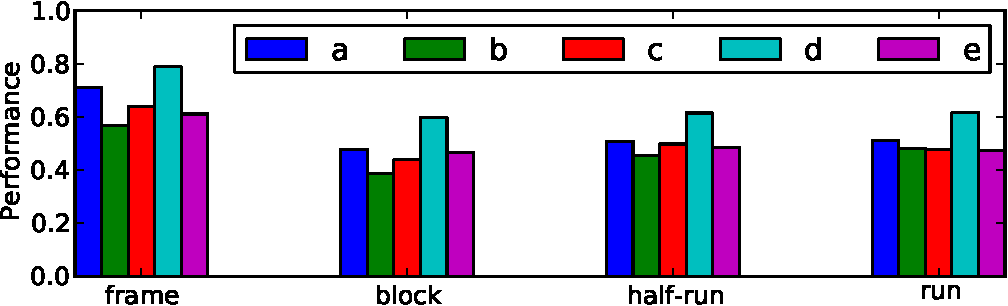
\includegraphics[width=\textwidth]{figures/svm-performance-graph}
\caption{}
\label{fig:svm-performance-graph}
\end{subfigure}
\begin{subfigure}{0.8\textwidth}
\centering
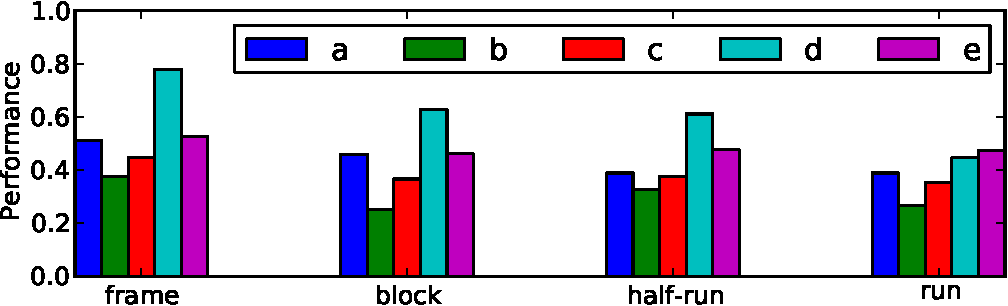
\includegraphics[width=\textwidth]{figures/nn-performance-graph}
\caption{}
\label{fig:nn-performance-graph}
\end{subfigure}
\caption{The performance estimates of the \subref{fig:svm-performance-graph} linear SVM and the \subref{fig:nn-performance-graph} feedforward neural network after cross-validation for all five subjects and four of the training and test split methods. }
\label{fig:performance-graph}
\end{figure*}

It is evident that, as the temporal delay between data in the training and test sets increases, the estimated performance of the classifiers decreases.
This relationship is plotted in figure \ref{fig:performance-verse-temporal-distance}.

\begin{figure}
\centering
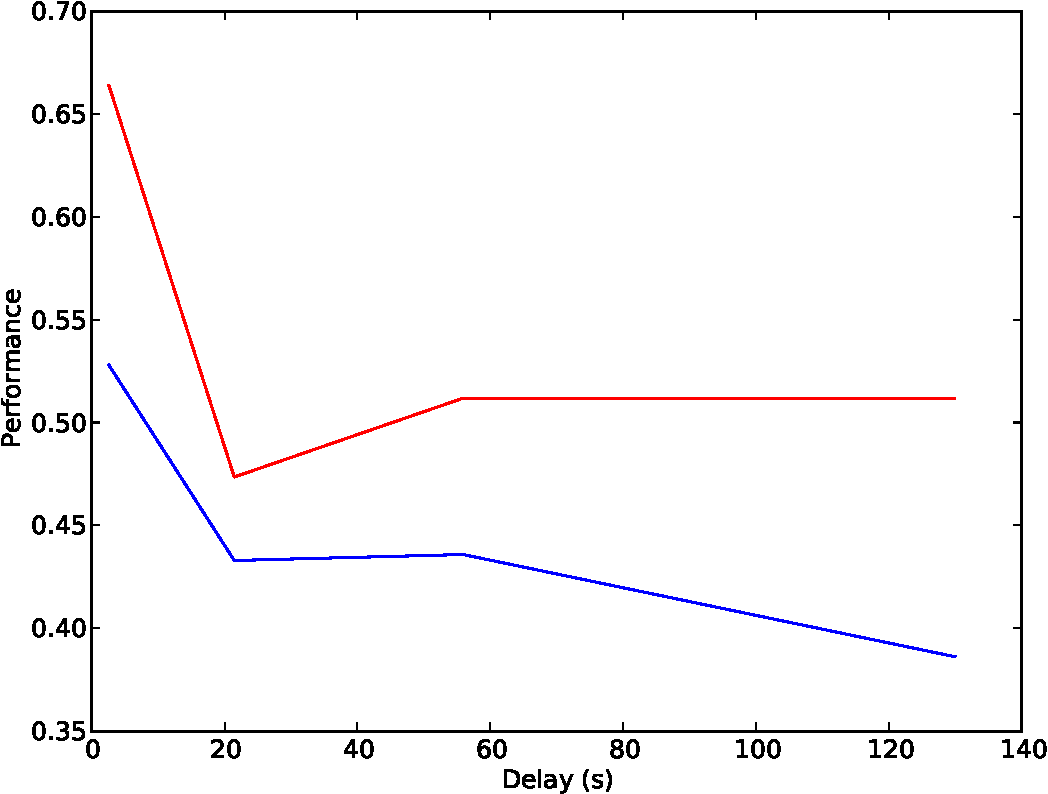
\includegraphics[width=0.3\textwidth]{figures/performance-verse-temporal-distance}
\caption{The average performance of the SVM and neural network classifiers plotted against the average temporal delay between data in the training and test sets.}
\label{fig:performance-verse-temporal-distance}
\end{figure}

The average confusion matrix presented in figure \ref{fig:average-confusion} gives a more intuitive look at the performance of the classifier.
From this matrix we can see that the classifiers are much better at detecting the presence of a single character than any other count.
In fact, there are almost no cases of confusion between 1 and 2 characters.
Apparently, these two situations evoke very different responses in the brain.
The rest of the character counts are distinguished with relatively equal accuracy,
except for a slightly larger tendency to mis-classify the 6 character presentation.
It should also be noted that the majority of the incorrect responses lay just off the main diagonal.
These responses correspond to the classifier being wrong by a single character in its classification.
For example, the machine learning algorithm classified a frame as containing 4 characters when it only contained 3 characters.
The estimated performance does not take the cardinality of the classes into account and considers mislabeling 1 character as 2 equivalent to mislabeling 1 character as 6 characters.
A soft measure of accuracy that takes the cardinality of the classes into consideration may be useful but the results are harder to interpret.
A confusion matrix gives us the advantages of the soft measure while providing an easily interpretable look into the performance of the classifiers.

\begin{figure}
\centering
\begin{subfigure}{0.3\textwidth}
\centering

\begin{tabular}{*{9}{c}}
& & \multicolumn{6}{c}{predicted count} & \\
& & 1 & 2 & 3 & 4 & 5 & 6 & \\
\multirow{6}{*}{\begin{sideways}actual count\end{sideways}}
& 1 & \cellcolor[rgb]{0.000000,1.000000,0.000000}75\% & \cellcolor[rgb]{0.987315,0.012685,0.000000}6\% & \cellcolor[rgb]{0.967214,0.032786,0.000000}8\% & \cellcolor[rgb]{0.995154,0.004846,0.000000}3\% & \cellcolor[rgb]{0.996400,0.003600,0.000000}3\% & \cellcolor[rgb]{0.991856,0.008144,0.000000}5\% & \cellcolor[rgb]{0.000000,1.000000,0.000000}71\%\\
& 2 & \cellcolor[rgb]{0.984543,0.015457,0.000000}6\% & \cellcolor[rgb]{0.000001,0.999999,0.000000}52\% & \cellcolor[rgb]{0.960568,0.039432,0.000000}9\% & \cellcolor[rgb]{0.793233,0.206767,0.000000}13\% & \cellcolor[rgb]{0.989269,0.010731,0.000000}5\% & \cellcolor[rgb]{0.754492,0.245508,0.000000}14\% & \cellcolor[rgb]{0.000002,0.999998,0.000000}50\%\\
& 3 & \cellcolor[rgb]{0.976984,0.023016,0.000000}7\% & \cellcolor[rgb]{0.946464,0.053536,0.000000}9\% & \cellcolor[rgb]{0.000000,1.000000,0.000000}53\% & \cellcolor[rgb]{0.228780,0.771220,0.000000}20\% & \cellcolor[rgb]{0.980048,0.019952,0.000000}7\% & \cellcolor[rgb]{0.995294,0.004706,0.000000}3\% & \cellcolor[rgb]{0.000001,0.999999,0.000000}51\%\\
& 4 & \cellcolor[rgb]{0.992536,0.007464,0.000000}4\% & \cellcolor[rgb]{0.888490,0.111510,0.000000}11\% & \cellcolor[rgb]{0.154156,0.845844,0.000000}21\% & \cellcolor[rgb]{0.000336,0.999664,0.000000}37\% & \cellcolor[rgb]{0.500333,0.499667,0.000000}17\% & \cellcolor[rgb]{0.939464,0.060536,0.000000}10\% & \cellcolor[rgb]{0.000499,0.999501,0.000000}36\%\\
& 5 & \cellcolor[rgb]{0.995930,0.004070,0.000000}3\% & \cellcolor[rgb]{0.976984,0.023016,0.000000}7\% & \cellcolor[rgb]{0.934220,0.065780,0.000000}10\% & \cellcolor[rgb]{0.299381,0.700619,0.000000}19\% & \cellcolor[rgb]{0.000001,0.999999,0.000000}50\% & \cellcolor[rgb]{0.919415,0.080585,0.000000}11\% & \cellcolor[rgb]{0.000000,1.000000,0.000000}55\%\\
& 6 & \cellcolor[rgb]{0.917261,0.082739,0.000000}11\% & \cellcolor[rgb]{0.217071,0.782929,0.000000}20\% & \cellcolor[rgb]{0.994473,0.005527,0.000000}4\% & \cellcolor[rgb]{0.888730,0.111270,0.000000}11\% & \cellcolor[rgb]{0.880363,0.119637,0.000000}12\% & \cellcolor[rgb]{0.000031,0.999969,0.000000}43\% & \cellcolor[rgb]{0.000004,0.999996,0.000000}48\%\\
&   & \cellcolor[rgb]{0.000000,1.000000,0.000000}75\% & \cellcolor[rgb]{0.000001,0.999999,0.000000}52\% & \cellcolor[rgb]{0.000000,1.000000,0.000000}53\% & \cellcolor[rgb]{0.000336,0.999664,0.000000}37\% & \cellcolor[rgb]{0.000001,0.999999,0.000000}50\% & \cellcolor[rgb]{0.000031,0.999969,0.000000}43\% & \cellcolor[rgb]{0.000001,0.999999,0.000000}52\%\\
\end{tabular}

\caption{}
\label{fig:average-confusion-svm}
\end{subfigure}
\begin{subfigure}{0.3\textwidth}
\centering

\begin{tabular}{*{8}{c}}
& & \multicolumn{6}{c}{predicted count} \\
& & 1 & 2 & 3 & 4 & 5 & 6 \\
\multirow{6}{*}{\begin{sideways}actual count\end{sideways}}
& 1 & \cellcolor[rgb]{0.000000,1.000000,0.000000}62\% & \cellcolor[rgb]{0.975443,0.024557,0.000000}7\% & \cellcolor[rgb]{0.841309,0.158691,0.000000}12\% & \cellcolor[rgb]{0.971887,0.028113,0.000000}8\% & \cellcolor[rgb]{0.997938,0.002062,0.000000}1\% & \cellcolor[rgb]{0.960675,0.039325,0.000000}9\%\\
& 2 & \cellcolor[rgb]{0.933406,0.066594,0.000000}10\% & \cellcolor[rgb]{0.000009,0.999991,0.000000}46\% & \cellcolor[rgb]{0.933406,0.066594,0.000000}10\% & \cellcolor[rgb]{0.831816,0.168184,0.000000}13\% & \cellcolor[rgb]{0.989177,0.010823,0.000000}5\% & \cellcolor[rgb]{0.569328,0.430672,0.000000}16\%\\
& 3 & \cellcolor[rgb]{0.979969,0.020031,0.000000}7\% & \cellcolor[rgb]{0.960675,0.039325,0.000000}9\% & \cellcolor[rgb]{0.000018,0.999982,0.000000}44\% & \cellcolor[rgb]{0.071219,0.928781,0.000000}23\% & \cellcolor[rgb]{0.984753,0.015247,0.000000}6\% & \cellcolor[rgb]{0.902345,0.097655,0.000000}11\%\\
& 4 & \cellcolor[rgb]{0.989896,0.010104,0.000000}5\% & \cellcolor[rgb]{0.919227,0.080773,0.000000}11\% & \cellcolor[rgb]{0.159047,0.840953,0.000000}21\% & \cellcolor[rgb]{0.001187,0.998813,0.000000}34\% & \cellcolor[rgb]{0.739428,0.260572,0.000000}14\% & \cellcolor[rgb]{0.586267,0.413733,0.000000}16\%\\
& 5 & \cellcolor[rgb]{0.990567,0.009433,0.000000}5\% & \cellcolor[rgb]{0.971887,0.028113,0.000000}8\% & \cellcolor[rgb]{0.933406,0.066594,0.000000}10\% & \cellcolor[rgb]{0.333341,0.666659,0.000000}18\% & \cellcolor[rgb]{0.000017,0.999983,0.000000}44\% & \cellcolor[rgb]{0.697341,0.302659,0.000000}15\%\\
& 6 & \cellcolor[rgb]{0.945244,0.054756,0.000000}10\% & \cellcolor[rgb]{0.811482,0.188518,0.000000}13\% & \cellcolor[rgb]{0.937595,0.062405,0.000000}10\% & \cellcolor[rgb]{0.667251,0.332749,0.000000}15\% & \cellcolor[rgb]{0.902345,0.097655,0.000000}11\% & \cellcolor[rgb]{0.000049,0.999951,0.000000}41\%\\
\end{tabular}

\caption{}
\label{fig:average-confusion-nn}
\end{subfigure}
\caption{The average confusion matrices for the \subref{fig:average-confusion-svm} SVM and \subref{fig:average-confusion-nn} neural network classifiers across all subjects using the block split.}
\label{fig:average-confusion}
\end{figure}

Sensitivity maps show a preponderance of classification sensitivity in
lateral occipital areas, ventral retinotopic early visual areas, and dorsal parietal lobe (figure \ref{fig:individual-sensitivity}). 
Individual subjects also displayed small regions of high sensitivity in idiosyncratic portions of temporal and frontal cortex. 
Specifically, classifier sensitivity was most affected by, in order of importance, lateral occipital regions, lingual areas, and dorsal parietal lobe (table \ref{tab:full-sensitivity}). 

\begin{figure*}
\centering
\begin{subfigure}{0.3\textwidth}
\centering
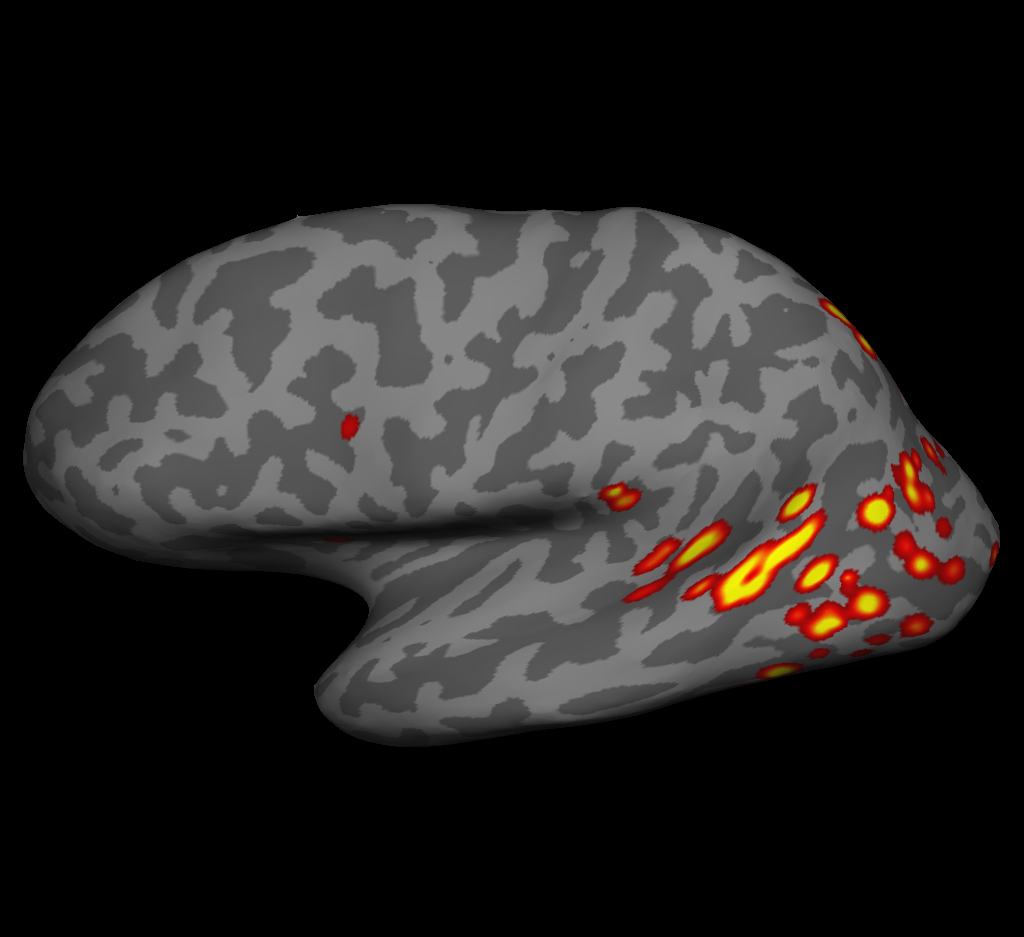
\includegraphics[width=\textwidth]{figures/s1-lh-lateral-sensitivity}
\caption{}
\end{subfigure}
\begin{subfigure}{0.3\textwidth}
\centering
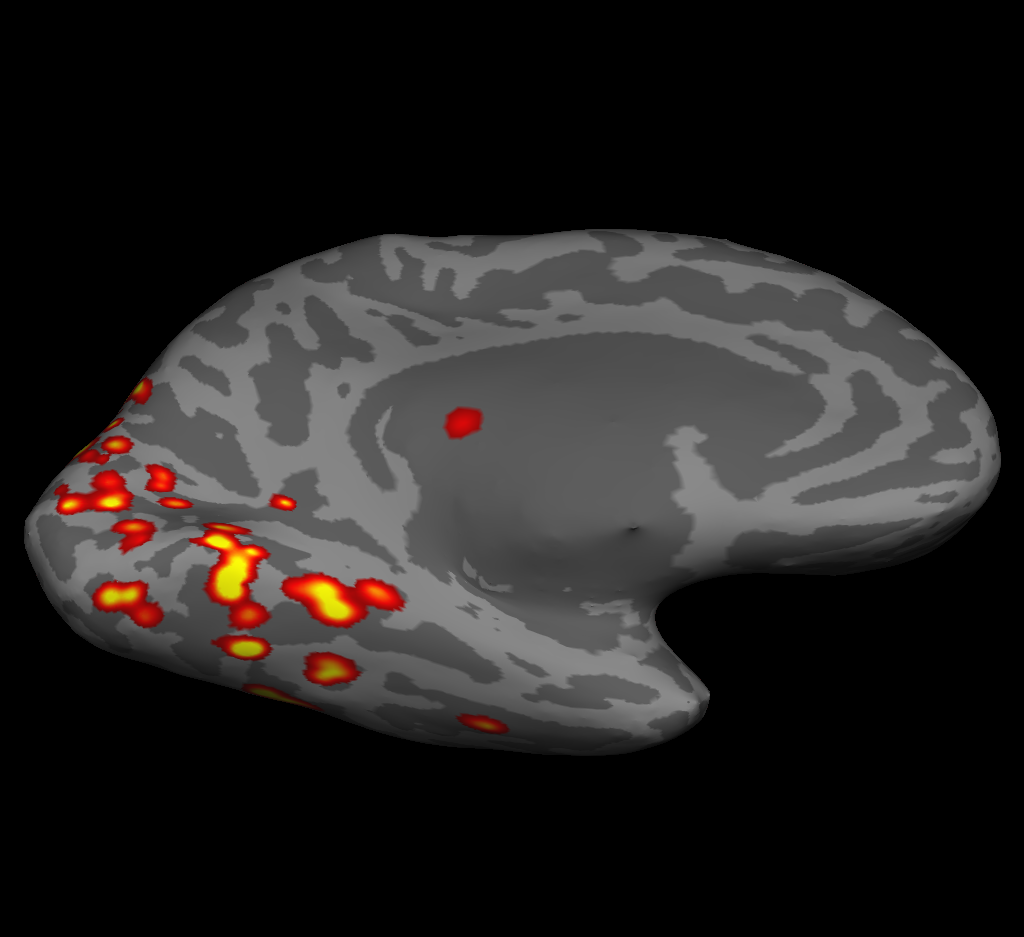
\includegraphics[width=\textwidth]{figures/s1-lh-medial-sensitivity}
\caption{}
\end{subfigure}
\begin{subfigure}{0.3\textwidth}
\centering
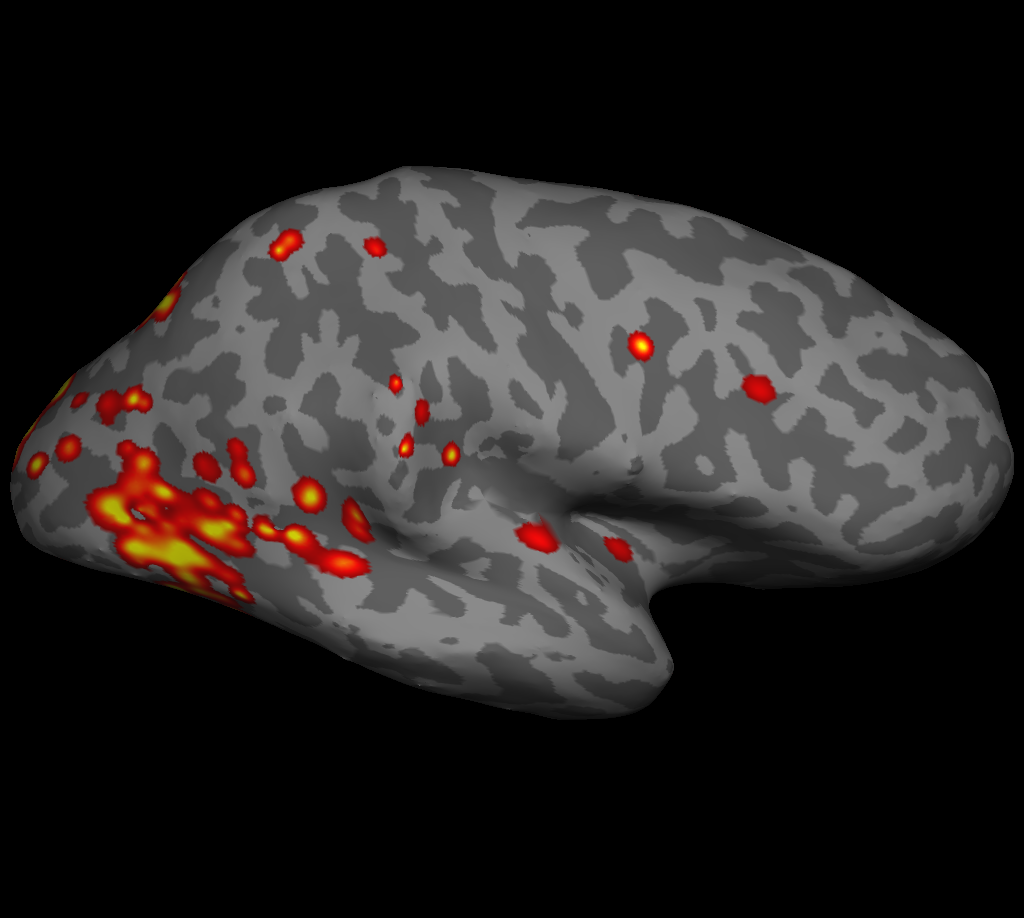
\includegraphics[width=\textwidth]{figures/s2-rh-lateral-sensitivity}
\caption{}
\end{subfigure}
\begin{subfigure}{0.3\textwidth}
\centering
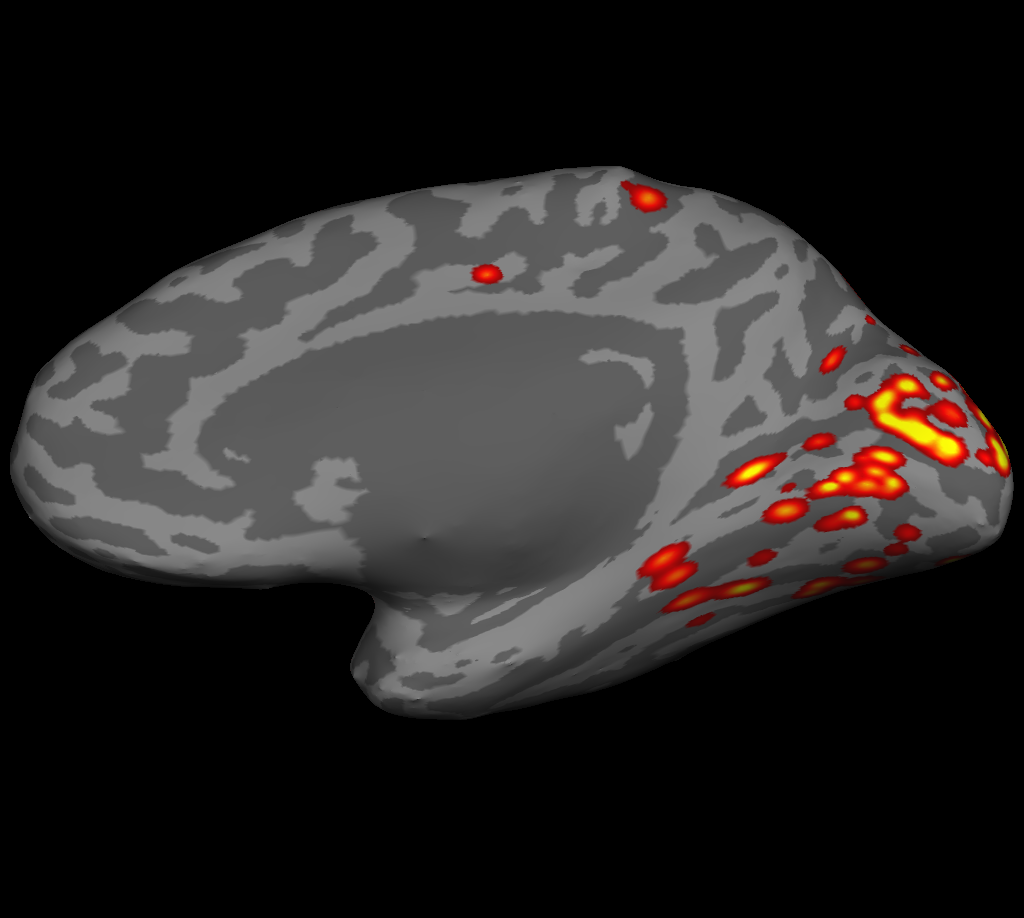
\includegraphics[width=\textwidth]{figures/s2-rh-medial-sensitivity}
\caption{}
\end{subfigure}
\begin{subfigure}{0.3\textwidth}
\centering
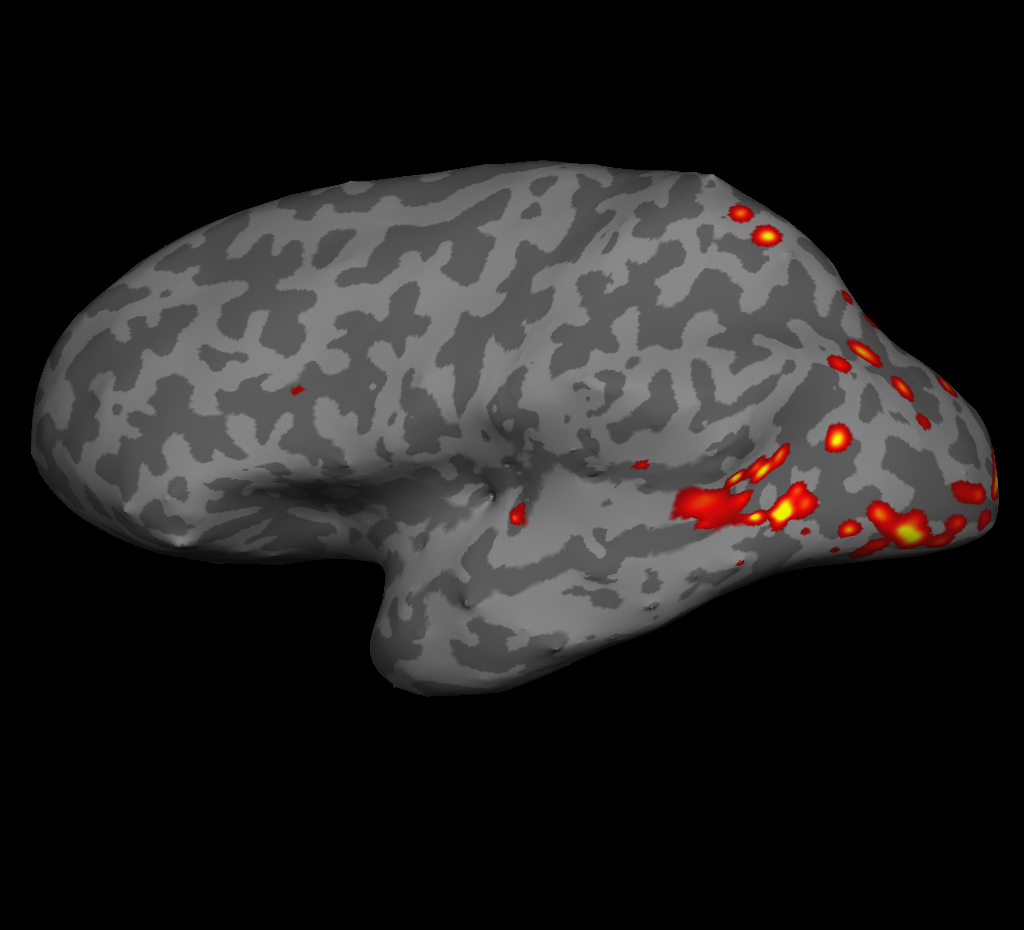
\includegraphics[width=\textwidth]{figures/s3-lh-lateral-sensitivity}
\caption{}
\end{subfigure}
\begin{subfigure}{0.3\textwidth}
\centering
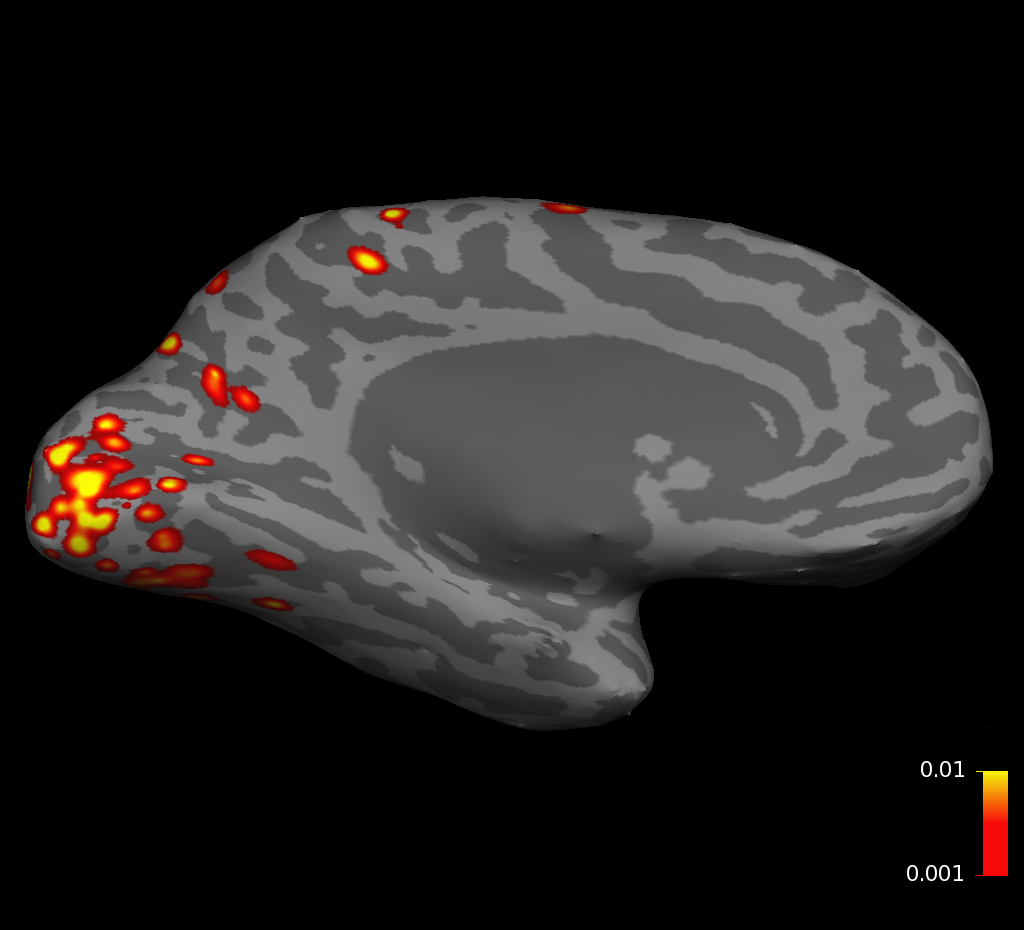
\includegraphics[width=\textwidth]{figures/s3-lh-medial-sensitivity}
\caption{}
\end{subfigure}
\caption{Individual sensitivity maps for three different subjects. 
The left hemisphere is presented for the first and third subjects while the right hemisphere is presented for the second subject.}
\label{fig:individual-sensitivity}
\end{figure*}

\begin{table*}
\centering

\begin{tabular}{cccccccc}
\toprule
Region & A & B & C & D & E  & Mean & Confidence Interval\\
\midrule
right lateral occipital & 26.54 & 13.41 & 16.26 & 24.17 & 26.49 & 21.37 & 18.76--23.98 \\
left lateral occipital & 13.37 & 25.65 & 15.37 & 24.02 & 25.75 & 20.83 & 18.37--23.28 \\
left superior parietal & 3.36 & 0.33 & 3.66 & 3.85 & 6.11 & 3.46 & 2.76--4.26 \\
left inferior parietal & 2.88 & 5.43 & 7.08 & 5.47 & 5.36 & 5.24 & 4.73--5.78 \\
right lingual & 6.64 & 5.96 & 10.30 & 5.88 & 5.25 & 6.81 & 5.93--7.69 \\
right superior parietal & 3.12 & 5.98 & 2.54 & 7.14 & 4.87 & 4.73 & 3.93--5.53 \\
right inferior parietal & 1.76 & 6.96 & 0.81 & 1.68 & 4.56 & 3.16 & 2.12--4.21 \\
left pericalcarine & 7.07 & 0.29 & 2.29 & 3.79 & 3.87 & 3.46 & 2.45--4.49 \\
left lingual & 8.63 & 8.38 & 10.09 & 4.92 & 3.50 & 7.10 & 6.07--8.37 \\
right superior temporal & 0.91 & 0.83 & 0.98 & 2.18 & 2.62 & 1.50 & 1.16--1.85 \\
right middle temporal & 0.23 & 0.84 & 6.08 & 1.69 & 2.54 & 2.28 & 1.28--3.27 \\
right pericalcarine & 4.64 & 5.99 & 6.02 & 0.40 & 2.20 & 3.85 & 2.82--4.91 \\
left superior temporal & 3.15 & 0.00 & 1.72 & 2.17 & 1.82 & 1.77 & 1.34--2.23 \\
right fusiform & 2.43 & 3.42 & 3.19 & 3.51 & 1.42 & 2.79 & 2.43--3.17 \\
right cuneus & 0.77 & 4.89 & 1.36 & 0.12 & 1.24 & 1.68 & 0.86--2.51 \\
left cuneus & 2.60 & 4.15 & 2.11 & 0.13 & 0.85 & 1.97 & 1.31--2.63 \\
left inferior temporal & 0.04 & 0.00 & 0.46 & 0.66 & 0.83 & 0.40 & 0.24--0.55 \\
right inferior temporal & 3.65 & 1.44 & 0.96 & 3.43 & 0.64 & 2.02 & 1.43--2.58 \\
left fusiform & 2.67 & 1.12 & 6.24 & 4.48 & 0.08 & 2.92 & 1.89--3.94 \\
left middle temporal & 5.53 & 4.93 & 2.51 & 0.33 & 0.00 & 2.66 & 1.62--3.70 \\
\bottomrule
\end{tabular}

\caption{Sensitivity values integrated across cortical surface labels.}
\label{tab:full-sensitivity}
\end{table*}

\section{Discussion}
VR environments provide a framework for creating  complex and dynamic stimuli in a controlled fashion while MVPA allows for the interrogation of neural-processing pathways when the underlying processing model is unknown.
When used together, VR stimuli and MVPA allow for the creation of very powerful experimental designs.
We have explored the benefits and potential pitfalls of these techniques and applied them to analyze the perception of the number of human characters presented in a natural scene.
The VR stimuli allowed us to generate natural stimuli while controlling the number of human characters presented and MVPA allowed us to interrogate the neural representation of this information without an a priori model.

The discriminative models learned by both the SVM and NN had a prediction accuracy that was 3--4 times above chance for all subjects.
Although both classifiers performed at well above chance levels for all subjects, the average performance on individual subjects varied significantly.
These variations could be the result of differences in age, general cognitive state, or simply how much attention the subject was paying to the stimulus during the scan.
The lack of a task during our stimulus makes these variations difficult to interpret since attention and cognitive state are not well controlled.
In future experiments, we plan to introduce a difficult task for the subjects to perform and we expect to see the average performance increase and the variation between subjects decrease.
However, the fact that the classifiers could still perform at well above chance levels without a focused task increases our confidence in the results.
In general, the classification accuracy of a particular number of perceived human characters decreased as the number of characters presented increased.
This effect is quite evident from the confusion matrix.
This results seems to be in agreement with the logarithmic nature of perception; i.e., it is easier to tell the difference between 1 and 2 characters than it is to tell the difference between 5 and 6 characters.
However, there is an interesting exception to this general trend.
There is a significant increase in confusion between 2 and 6 characters.
Again, this effect is quite evident from the confusion matrix.
This could be a result of 6 characters being too much for the subject to consider individually and the subject perceives 2 groups of characters rather than 6 individual characters.

This estimated prediction accuracy was calculated after correcting for the bias introduced by temporal correlations in the bold signal while minimizing variance.
As we have shown, decreasing the average temporal distance between examples in the training and test sets results in a less optimistically biased estimate of the classifier's performance.
However, the larger the average temporal distance enforced between the training and test sets the fewer possible folds exist for crossfold-validation which results in an estimate with a higher variance.
By characterizing the relationship between the average minimum temporal distance between the training and test sets and estimated classifier performance, we have found that the estimated performance reaches a minimum around 20 seconds.
These findings are consistent with our knowledge of the hemodynamic response.
That is, so long as the frames are separated by approximately the time-scale of the HRF then they can reasonably be considered independent, and this separation produces an appropriately conservative measure of classification performance. 
However, it is interesting that slightly better performance may be obtained for somewhat longer delays.
Many experiments separate their folds for crossfold-validation along runs.
While this ensures a sufficient temporal separation between training and test set examples, it also reduces the total number of folds available and thus increases the variance of the estimate.
Instead, we recommend splitting the data along whatever natural boundary of the experimental procedure is closest to, but not less than 20 seconds.

Ideally we would like to train our classifiers using data from the whole brain.
In this way, our analysis will not miss any relevant interactions that are not localized by our simple harmonic analysis.
Since MVPA is used in general when a good underlying model is not known, this is especially important.
However, the large number of voxels can then intractably confound the MVPA because
the number of training examples required to train a classifier generally increases exponentially with the number of dimensions.
One reason that the SVM is so popular and so effective in this field is that its performance is partially robust against insufficient training examples.
The simplicity of the SVM's discriminative model---a hyperplane---bounds the potential generalization error while the maximum-margin cost-function provides regularization.
Other researchers have already found that decreasing the dimensionality of the problem with various univariate measures, from percent activation to a one-way ANOVA, can be quite effective \citep{Norman2006,Pereira2009}.
However, most of these statistical stimulus-driven measures rely on a number of statistical assumptions about the underlying BOLD signal such as being normally distributed.
We have developed a technique, which we call harmonic analysis, that performs a similar role without making any assumptions about the signal.
While less appropriate for statistical analysis, we have found that harmonic analysis is an excellent tool for dimensionality reduction as a preprocessing step before MVPA.

The performance of our classifiers indicates that their is sufficient information in the pattern of BOLD signals to decode character count in a freely viewed stimulus. 
The results also suggest that the neural circuits that encode such information are both distributed and redundant.
In order to explore where in the brain this information is encoded, we developed a sensitivity mapping technique.
This technique allowed us to identify a small distributed subset of voxels that are sufficient for decoding perceived character count.
Using dimensionality reduction via harmonic analysis, we initially begin classification with 2000 voxels.
Using sensitivity analysis, we could then identify a subset of voxels an order of magnitude smaller that can be used for decoding with nearly the same accuracy as the full set.
This could indicate that only a small number of voxels are relevant for classification, or that the information is highly redundant between voxels, or, most likely, some a combination of these two.
Specifically, the harmonic analysis will select some voxels that covary with the stimulus, but their patterns of activation may not be highly discriminative with respect to character count.
These voxels will also be assigned low sensitivity values by the trained classifiers.
On the other hand, brain responses themselves can show strong spatial correlations on the centimeter scale, particularly in the higher-order visual areas that dominate our sensitivity results \citep{Engel1997}. 
Voxels sampling these regions could all show similar classification sensitivity, but yield redundant information.
Therefore, high sensitivity is sufficient but not necessary for the localization of a function in a particular region.

%\emph{The following two sentences were originally in the Introduction. I've moved it here to the Discussion, but it needs to be expanded. Write a few sentences that explain how our approach is different and better than the searchlight scheme. Are there any other competitors?} This sensitivity analysis employs an iterative approach to identify a sparse and potentially distributed set of voxels that are highly discriminative.
%This analysis can be contrasted to the popular ``searchlight'' technique which only evaluates small localized sets of voxels \citep{Kriegeskorte2006}.

When examined in conjunction with existing vision and cognitive neuroscience experiments, the sensitivity maps reveal insights as to how this information may be processed in the brain (Table 1).
By far, the most sensitivity (42\%) and therefore the most relevant mutual information is contained in the lateral occipital region (LO).
This region is most commonly associated with high level object recognition \citep{Grill-Spector2001}.
This is in contrast to the comparatively weak sensitivity (5.7\%) observed in upon the fusiform gyrus, which is also associated with object classification tasks and in particular the perception of human faces \citep{Kanwisher1997}.
Additionally, there is substantial sensitivity contained in low level retinotopic visual areas. The pericalcarine, lingual, and cuneus areas altogether account for 25\% of the observed sensitivity. The more ventral lingual areas contribute more strongly (13.9\%) then cuneus (3.7\%).
This is somewhat surprising given that the relevant information in the scene is not necessarily retinotopically organized given the randomized arrangement of buildings and characters as well as the free-viewing paradigm.
The presence of sensitivity in early, retinotopic visual areas, together with the preponderance of sensitivity in lateral-occipital areas may reflect the importance of retinotopic organization in the decoding of group size. LO combines both object-selectivity with retinotopic specificity \citep{Sayres2008}. Different group sizes could evoke complex but stereotypical patterns of responses in LO and other retinotopically organized areas as subjects visually interrogate the stimuli. Ventral early visual areas apparently also contribute to this information. The less retinotopic fusiform regions \citep{Schwarzlose2008,Sayres2010} also appear to less useful for decoding character number.
Substantial sensitivity (16.6\%) is also present in dorsal parietal cortex. The sensitivity along the dorsal stream suggests that the perception of motion and position are also useful for decoding subject number from our complex and dynamic VR stimuli.
As expected, something as abstract as the number of perceived human characters is not contained in a single voxel but rather is encoded in a distributed manner across many different visual processing areas working together.
Encouragingly, the sensitivity maps were consistent across subjects despite the lack of a controlled task.

There are some potential pitfalls in our approach that must be avoided, such as increased design complexity and difficulty of interpretation. 
Here, we have offered some initial tools and analyses to deal with these limitations, but further work is clearly needed.
Moreover, VR environments do carry some disadvantages over simpler dynamic stimuli such as prerecorded movies. Recording a movie is typically easier than programming a VR environment and movies can have a more realistic appearance than VR environments.
Additionally, the results presented in \cite{Han2005} indicate that there is some divergence in the way the brain processes real, that is recorded, and virtual visual worlds. 
However, cartoons were used to represent virtual visual worlds in this study, and it is likely that as the realism of VR environments increases this divergence in processing will decrease

Complex and dynamic stimuli allow researchers to examine neural processing in a more natural state and VR environments make it easier to design and control such stimuli.
MVPA allows researchers to explore the coding of information in the brain when an underlying model is not already known and to discover new and interesting interactions.
Used together, VR stimuli and MVPA allow for novel and valuable experimental designs.
Altogether, our results suggest that the combination of VR with machine-learning analysis schemes will offer a fruitful new tool for the analysis of brain responses in stimulus scenarios that more closely resemble natural human experience.

\bibliography{bib}

\end{document}
